%! Author = izmir_lcz_deep_morphology_mert_yavas
%! Target = Sustainable Cities and Society, with CEUS / Urban Climate backups
%! CRS = to be locked in docs/methodology/pre_analysis_lock_2026-06-14.md

\documentclass[review,1p]{elsarticle}

\usepackage{mypreamble}
\usepackage{setspace}
%% Acronym definitions loaded before the manuscript body.

\acrodef{LCZ}{Local Climate Zone}
\acrodef{DSM}{surface model}
\acrodef{DTM}{Digital Terrain Model}
\acrodef{nDSM}{normalized surface model}
\acrodef{SVF}{Sky View Factor}
\acrodef{LST}{Land Surface Temperature}
\acrodef{NDVI}{Normalized Difference Vegetation Index}
\acrodef{NDBI}{Normalized Difference Built-up Index}
\acrodef{NDWI}{Normalized Difference Water Index}
\acrodef{GEE}{Google Earth Engine}
\acrodef{OSM}{OpenStreetMap}
\acrodef{CRS}{Coordinate Reference System}
\acrodef{FUR}{Functional Urban Region}
\acrodef{CNN}{Convolutional Neural Network}
\acrodef{ViT}{Vision Transformer}
\acrodef{MLP}{Multilayer Perceptron}
\acrodef{RF}{Random Forest}
\acrodef{SHAP}{SHapley Additive exPlanations}
\acrodef{XAI}{Explainable Artificial Intelligence}
\acrodef{CV}{Cross-Validation}
\acrodef{MAUP}{Modifiable Areal Unit Problem}
\acrodef{ARI}{Adjusted Rand Index}
\acrodef{F1}{F1-score}
\acrodef{MCC}{Matthews Correlation Coefficient}
\acrodef{RMSE}{Root Mean Square Error}
\acrodef{MAE}{Mean Absolute Error}


\journal{Sustainable Cities and Society}

\begin{document}

    \graphicspath{{../../figures/main/}{../../figures/supplementary/}}

    \begin{frontmatter}

\title{Climorfa: Climate-Sensitive Urban Morphology in Izmir}

\author[1]{Yusuf Emino\u{g}lu\corref{cor1}\fnref{orcidYusuf}}
\ead{yusuf.eminoglu@deu.edu.tr}
\author[1]{Mert Yava\c{s}\fnref{orcidMert}}
\author[1]{Hilmi Evren Erdin\fnref{orcidHilmi}}
\author[2]{\c{S}\i rk\i \fnref{orcidEsra}}
\cortext[cor1]{Corresponding author.}
\fntext[orcidYusuf]{ORCID: \href{https://orcid.org/0009-0005-6000-2934}{0009-0005-6000-2934}}
\fntext[orcidMert]{ORCID: \href{https://orcid.org/0009-0001-0477-2599}{0009-0001-0477-2599}}
\fntext[orcidHilmi]{ORCID: \href{https://orcid.org/0000-0002-3350-8930}{0000-0002-3350-8930}}
\fntext[orcidEsra]{ORCID: \href{https://orcid.org/0000-0001-7914-4821}{0000-0001-7914-4821}}
\address[1]{Department of City and Regional Planning, Dokuz Eyl\"ul University, \.{I}zmir, T\"urkiye}
\address[2]{Department of City and Regional Planning, Siirt University, Siirt, T\"urkiye}

\begin{abstract}
Local Climate Zones (LCZs) provide a transferable climate-form vocabulary, but
locally actionable interpretation requires finer morphological evidence,
transparent scale choices, and spatially independent validation. We assembled
an analysis-ready 250 m grid for the Izmir functional urban region containing
16,506 grid units and 374 fields from a local 5 m surface model,
building and street geometry, Sentinel-2, Landsat 8/9 land-surface temperature
(LST), Dynamic World, ESA WorldCover, canopy height, coastal context, OpenStreetMap
(OSM), and 2024 population demand. Global LCZ labels were treated as weak labels.
The present analysis retained 5,339 grid units from LCZ 3, 6, 8, and
9 at confidence $\geq 0.60$. LightGBM, XGBoost, Random Forest, and Extra Trees
models were evaluated with five stratified 1.25 km spatial-block folds. Additive ablations tested
morphology, vegetation, green-blue context, full proxy context, and network-cost
two-step floating catchment area (2SFCA) green-space access at 400, 800, and
1,200 m. The primary 800 m LightGBM model achieved macro-F1 0.838, compared
with 0.663 for morphology alone; XGBoost, Random Forest, and Extra Trees reached
0.835, 0.829, and 0.819, respectively, at the primary recipe. Adding vegetation
produced the largest early gain, while 800 m 2SFCA added 0.0056 macro-F1 to
LightGBM relative to an otherwise identical full-context model. LightGBM
leave-one-district-out macro-F1 averaged 0.723 across 11 districts (range
0.475--0.819), revealing substantial transfer heterogeneity. Weak LCZ classes
also differed in summer LST ($H=1592.0$, $\epsilon^2=0.298$); NDVI and canopy
volume were negatively associated with LST, whereas NDBI, building coverage,
and road density were positively associated. The 569-location manual audit was
completed; among 96 high-quality audited units in the four-class modeling population,
exact agreement was 8.3\% for both the weak labels and LightGBM, exposing strong
class-space compression. A municipal park inventory provided strong district-level
macro triangulation of OSM supply but not object-level validation. These findings
establish a reproducible, explainable baseline and show why surface-model structure,
vegetation, network accessibility, spatial transfer, and audit evidence must
accompany LCZ interpretation. Raster/figure-ground deep branches remain untrained,
so deep-fusion superiority is not claimed.
\end{abstract}

\begin{keyword}
    Local Climate Zones \sep urban morphology \sep surface model \sep
    land-surface temperature \sep two-step floating catchment area \sep
    spatial cross-validation \sep explainable machine learning \sep Izmir
\end{keyword}

\end{frontmatter}

\begin{figure}[H]
    \centering
    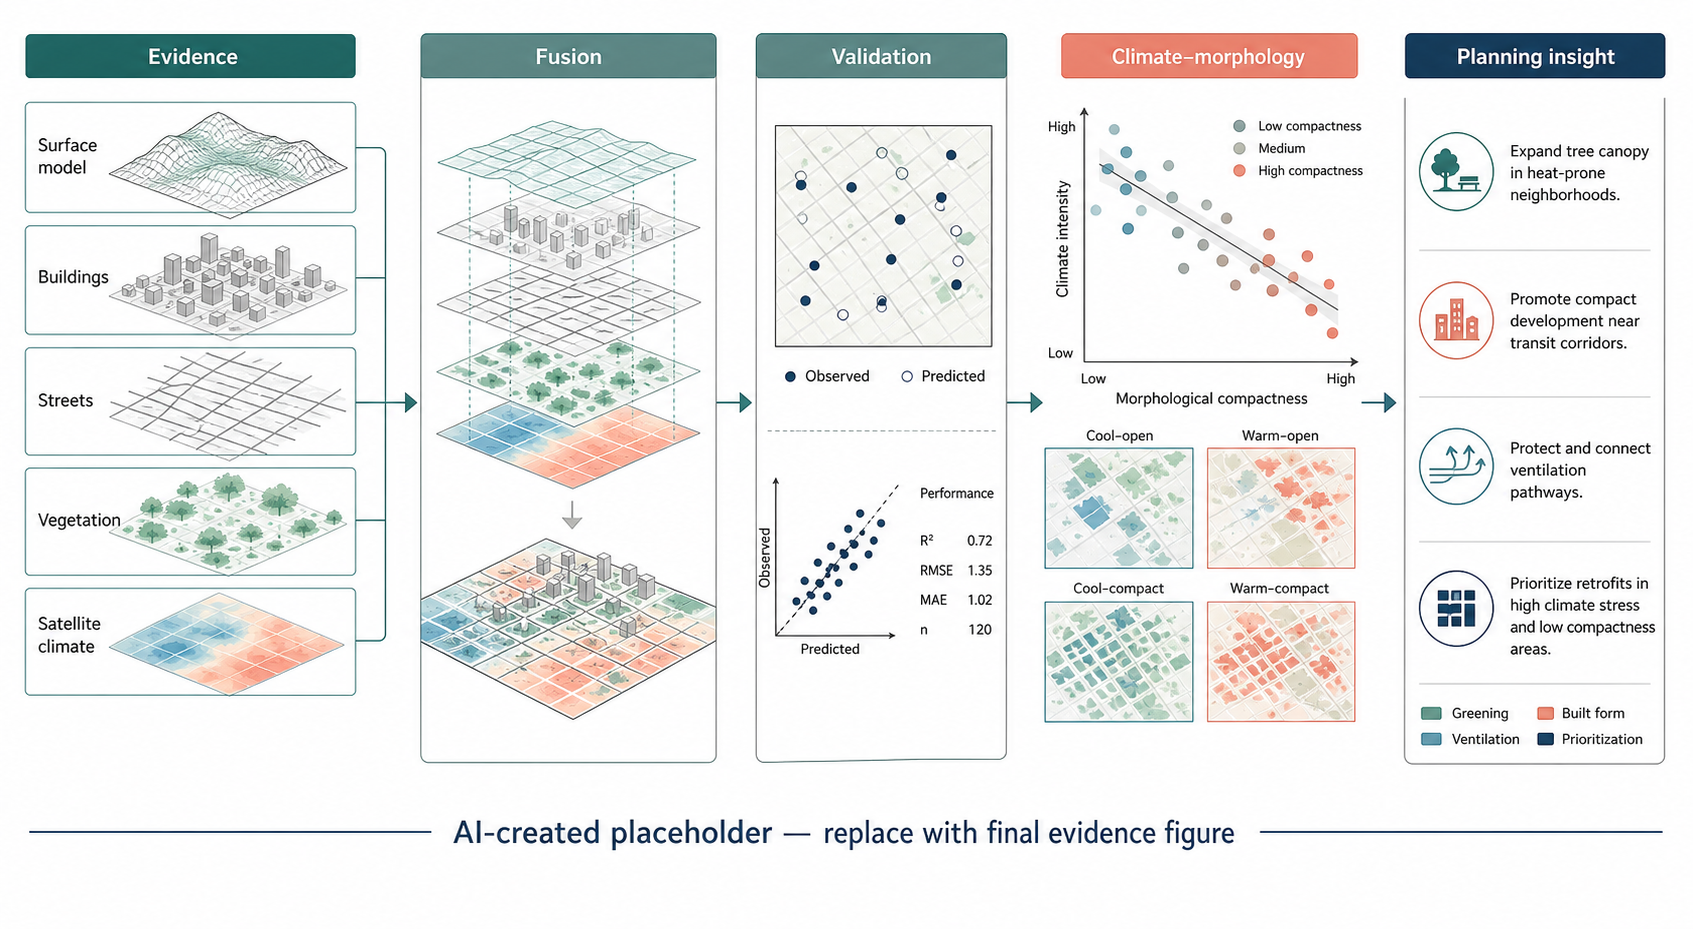
\includegraphics[width=\textwidth]{graphical_abstract.png}
    \caption*{Graphical abstract summarizing the Climorfa evidence workflow,
    from multisource 250 m feature integration through spatial validation,
    climate-response analysis, and audited-label comparison.}
\end{figure}



    \doublespacing
    \ifdefined\withlinenumbers
        \linenumbers
    \fi
    \acresetall

    \section{Introduction}\label{sec:introduction}

Urban heat is produced by interactions among surface materials, built form,
vegetation, moisture, radiation, ventilation, and human activity. The Local
Climate Zone (LCZ) framework made this complexity operational by defining a
standard climate-form vocabulary for urban temperature studies
\citep{stewart2012LocalClimate}. Earth-observation classification and the
Worldwide Urban Database and Access Portal Tools (WUDAPT) subsequently made
LCZ mapping repeatable across cities \citep{bechtel2012ClassifiLocal,
bechtel2015MappingLocal,ching2018WudaptUrban,bechtel2019GeneratiWudapt}, and a
a global LCZ product supports comparative urban and Earth-system analysis
\citep{demuzere2022GlobalLocal}. The framework is therefore indispensable for
comparability, but comparability is not the same as local planning resolution.

Within-class thermal variability has been observed across climates, cities,
seasons, and measurement systems \citep{geletic2016LandSurface,
skarbit2017EmployinUrban,kwok2019WellDoes,yang2020InvestigDiversit,
li2022VariabilLand}. This matters especially in coastal metropolitan regions,
where sea proximity, topographic transition, vegetation structure, and
contrasting compact, open, industrial, and peripheral fabrics may produce
substantial variation within a nominal LCZ. Recent work consequently relates
LST to two- and three-dimensional morphology, vegetation, and functional
context rather than treating class membership as a complete explanation
\citep{zhou2022UnderstaEffects,wang2023EffectivFactors,
zhou2023IdentifyEffects,liu2025UnveilinDifferen,yu2026UrbanMorpholo}. The
question is no longer only which LCZ occupies a location, but which measurable
features make locally similar labels climatically different.

Three methodological gaps remain. First, many classification pipelines learn
LCZ labels from multisource imagery but inherit label uncertainty and spatial
scale assumptions \citep{qiu2018FeatureImportan,yoo2019ComparisBetween,
qiu2020MultilevFeature,yoo2020ImprovinLocal,yan2022ComparinObject}. Second,
urban climate models can be accurate while remaining difficult to translate
into design action if 3D structure, street interface, vegetation volume, and
network context are compressed into opaque predictors. Third, random train-test
splits can reward spatial autocorrelation rather than transferable morphology;
grid and block comparisons show that analytical support changes estimated
form--temperature relationships \citep{jeon2023ImpactsUrban,wu2022ScaleEffect,
li2026InvestigEffect}. Explainability, spatial holdouts, and scale sensitivity
are therefore parts of the estimand, not optional presentation devices.

Izmir is a demanding test of this proposition. Its functional urban region
contains dense coastal districts, hillside settlement, open low-rise fabrics,
large-footprint industrial zones, suburban expansion, and fragmented
peripheral development. Coastal heat-risk interpretation must also account for
local vulnerability and the limits of transferring LCZ semantics between
cities \citep{canguzel2024ClimateChange,zhang2025ApplicabLocal}. We therefore
treat the global LCZ map as weak-label infrastructure and combine it with a
local 5 m surface model, exact building and road geometry, vegetation structure, remotely
sensed land cover and LST, coastal context, and competition-adjusted
network accessibility.

The study makes four evidence-backed contributions. First, it documents an
analysis-ready 250 m Izmir grid with explicit provenance, missingness,
collinearity, and proxy language. Second, it quantifies the incremental value
of morphology, surface-model structure, vegetation, green-blue context, and street-network
features under leakage-aware spatial cross-validation. Third, it replaces
Euclidean green-space buffers with a network-cost two-step floating catchment
area (2SFCA) measure and tests 400, 800, and 1,200 m thresholds. Fourth, it
connects weak-label morphology to LST, feature importance, uncertainty, and
leave-district-out transfer. This explanatory sequence follows the broader
principle that urban-form machine learning should connect prediction,
interpretation, and planning meaning \citep{karl2026RelationBetween}.

The analysis combines a prespecified 569-location manual audit with weak-label and tabular model evaluation. The audit provides a direct comparison between global labels, model predictions, and locally reviewed morphology, so the reported profiles and predictions are interpreted against observed local fabric.

    \section{Literature review}\label{sec:literature}

\subsection{LCZs as climate-form vocabulary and weak-label infrastructure}

LCZs were designed as physically interpretable classes for near-surface urban
climate comparison \citep{stewart2012LocalClimate}. Early remote-sensing
classification, monitoring-network design, and worldwide mapping established
the scheme as both a measurement vocabulary and a scalable mapping task
\citep{bechtel2012ClassifiLocal,lelovics2014DesignUrban,
bechtel2015MappingLocal}. WUDAPT extended that logic into a shared urban
modelling infrastructure, but comparisons with detailed GIS canopy parameters
also showed that class-based descriptions cannot reproduce every local
morphological quantity \citep{ching2018WudaptUrban,
hammerberg2018ImplicatEmployin,zonato2020EvaluatiPerforma}.

Classification performance depends on sensor, city, training data, object or
pixel support, and feature fusion. Random forests, convolutional networks,
residual networks, multilevel fusion, and multisource seasonal imagery have all
improved LCZ mapping \citep{qiu2018FeatureImportan,yoo2019ComparisBetween,
qiu2020MultilevFeature,yoo2020ImprovinLocal,wang2023LocalClimate}. Yet high
map accuracy does not remove uncertainty caused by incomplete buildings,
different urban forms, or transfer between climatic contexts
\citep{wang2018AssessinLocal,yoo2020ImprovinLocal,
yan2022ComparinObject}. Global mapping is therefore best treated as a
consistent prior whose local meaning must be checked, rather than as a complete
substitute for local labels \citep{demuzere2022GlobalLocal}.

Thermal separability is similarly conditional. Numerical, satellite, and
station evidence shows useful LCZ contrasts, but also within-class variation
and context sensitivity \citep{geletic2016LandSurface,skarbit2017EmployinUrban,
kwok2019WellDoes,yang2020InvestigDiversit}. Frontal area, vegetation, and
scenario definition can change class-level temperature patterns
\citep{li2022VariabilLand,zhou2023IdentifyEffects,
deng2024SensitivLocal}. Coastal-city risk research adds a transferability
warning: an LCZ may organize exposure, but it cannot on its own represent
vulnerability, accessibility, or local design opportunity
\citep{ma2023InvestigUrban,zhang2025ApplicabLocal}. These findings motivate our
weak-label terminology, confidence threshold, mixed-cell flag, and manual-audit
gate.

\subsection{Urban morphometrics, figure-ground form, and fabric typology}

Urban-climate mechanisms predate LCZ classification. Comparative studies linked
urban heat to form and thermal properties, while view-factor research formalized
how surrounding geometry controls radiative exposure \citep{emmanuel2007UrbanHeat,
chen2010ViewFactor}. Sky-view-factor footprints demonstrate that even a
seemingly local 3D metric has a spatial support that must be specified
\citep{middel2018ViewFactor}. Building density, compactness, height,
fragmentation, imperviousness, and vegetation consequently need to be measured
as a system rather than as interchangeable proxies.

Empirical studies have connected LST to building form, landscape configuration,
and multisource urban structure using regression and machine learning
\citep{ferreira2019ExplorinRelation,huang2019InvestigEffects,
sun2019QuantifyEffects,zhang2019EvaluatiEffect}. Later work strengthened the
3D component by evaluating vertical morphology, seasonal disparity, and
scale-dependent landscape patterns \citep{alexander2021InfluencProporti,
yang2021AssessinEffects,chen2022SeasonalDisparat,
han2022UnderstaSeasonal,wu2022QuantifyInfluenc,wu2022ScaleEffect}. The
consistent lesson is not that one feature universally dominates, but that
horizontal density, vertical structure, open space, and vegetation interact
across spatial supports.

Recent studies increasingly compare grid, block, functional-zone, and LCZ
supports. Grid--block differences have been demonstrated directly
\citep{jeon2023ImpactsUrban}; cumulative morphology, satellite/in-situ
comparison, and functional-zone analysis further show that aggregation choices
shape interpretation \citep{park2023QuantifyCumulati,puche2023InsightsInto,
du2024DoesUrban,lin2024DoesUrban}. Studies of stationarity, threshold effects, and urban-rural
or climate-zone differences caution against universal linear prescriptions
\citep{yuan2024EffectsUrban,zhao2024MechanisStationa,
chen2025ImpactsThreshol,debray2025UniversaPatterns}. This literature supports
our decision to report class profiles and transfer diagnostics rather than a
single pooled coefficient.

Three-dimensional green structure is equally important. Canopy amount,
vertical pattern, building--green interaction, and nature-based-solution scale
can modify cooling potential \citep{bai2025ImpactBuilding,
hu2025ComparinGreen,wei2025UrbanCooling}. Surface and canopy temperatures may
also respond differently to 2D and 3D morphology and to analytical scale
\citep{wu2025ContrastUrban,yu2026UrbanMorpholo}. We therefore distinguish
canopy cover, canopy height, and a canopy-volume proxy, while avoiding the claim
that any of them is measured biomass.

\subsection{Surface model, vegetation, and thermal mechanisms}

Surface-model information strengthens urban morphology by representing the combined
surface rather than footprints alone. Studies using LCZ, 2D/3D indicators,
SVF, and seasonal temperature consistently show that radiative openness and
vertical roughness contribute information beyond planimetric density
\citep{wang2018AssessinLocal,zhou2022UnderstaEffects,
ma2024XgboostBased,wang2025SeasonalEffects}. However, a surface model is not automatically
a building-height model. Terrain, vegetation, bridges, water artefacts, and
vertical datum uncertainty must be separated from built-form interpretation.
Our 5 m surface model is therefore used through surface-elevation range and standard
deviation together with independently derived floor-count height proxies.

Vegetation can affect temperature through shade, evapotranspiration, and
surface-energy partitioning, but effects depend on vegetation structure,
background climate, urban form, and season. Evidence spans phenology,
class-specific surface temperature, green-roof scenarios, and urban cooling
across nature-based-solution types \citep{kabano2021EvidenceUrban,
wang2023EffectivFactors,sanchez2025AssessinSpatial,wei2025UrbanCooling}.
Accordingly, vegetation enters both the classification ablation and the climate
response analysis, while causal cooling claims are excluded from cross-sectional
correlations.

\subsection{Deep learning and explainable urban-climate models}

Deep learning is useful when raster texture and figure-ground configuration
contain information that tabular summaries cannot preserve. LCZ research has
shown gains from residual CNNs, multilevel feature fusion, and combinations of
incomplete buildings with Sentinel imagery \citep{qiu2018FeatureImportan,
qiu2020MultilevFeature,yoo2020ImprovinLocal}. Multi-view urban-fabric models
extend this idea beyond a single overhead image and across spatial scales
\citep{fang2024UrbanclaDeep}. These advances motivate CLIMORFA's planned raster
and figure-ground branches.

Prediction alone is insufficient. XGBoost, CatBoost, SHAP, automated machine
learning, unsupervised clustering, and nonlinear models increasingly expose
thresholds, interactions, and geographically varying effects
\citep{ma2024XgboostBased,liu2025UnveilinDifferen,
xu2025CharacteThermal,wang2025RevealinImpact,
liu2026UnderstaNonlinea,wan2026AnalyzinImpact}. Interpretive frameworks also
emphasize mechanisms and seasonal differences rather than a ranking of feature
importance alone \citep{han2025PerspectUndersta,
wang2025SeasonalEffects}. We therefore report tree importance only as a first
explanation and require SHAP plus spatially explicit neural attribution before
any final deep-model claim. The general analogue is explainable urban-form
machine learning that connects model evidence to planning interpretation
\citep{karl2026RelationBetween}.

\subsection{Grid scale, network context, and spatial validation}

Scale is a substantive uncertainty. The support of SVF, urban form, green
pattern, and temperature changes the observed relationship
\citep{middel2018ViewFactor,wu2022ScaleEffect,hu2025ComparinGreen,
li2026InvestigEffect}. Urban mobility and heat exposure also operate along
networks rather than through Euclidean circles \citep{zhang2025MobilitiHeat}.
For green-space supply, a buffer counts nearby area but ignores network cost,
population competition, and shared destinations. We therefore use a network
2SFCA and retain 400/800/1,200 m thresholds as explicit sensitivity parameters.

Spatial validation is the companion requirement. Typology and climate studies
can exploit regional texture, city identity, or neighbourhood autocorrelation
unless folds are spatially separated. Comparing spatial blocks and held-out
districts provides a more demanding test of transfer. It also reveals when
apparently strong average performance hides local failure. Finally, climate
vulnerability cannot be inferred from morphology alone: heat risk, perceived
stress, and composite vulnerability combine exposure with social sensitivity
and adaptive capacity \citep{mashhoodi2024UrbanForm,iqbal2025DoesPerceive,
turner2025DevelopmValidati}. Our planning interpretation is therefore confined
to morphology and access signals and does not label vulnerable populations.



    \section{Study area and data}\label{sec:study_area_data}

\subsection{Izmir functional urban region and analytical support}

The study area is the operational Izmir functional urban region (FUR), not a
single municipality or a selectively drawn urban core. This choice preserves
the connected metropolitan system in which dense central and coastal apartment
fabrics, hillside and peripheral settlement, large low-rise industrial areas,
port and airport functions, suburban expansion, agricultural transition, and
green-blue systems coexist. The coastal setting is analytically important
because local heat-risk interpretation can differ from inland cities and must
not be reduced to urban form alone \citep{canguzel2024ClimateChange,
zhang2025ApplicabLocal}.

All vector and raster analyses were harmonized to EPSG:5253. The primary support
is a 250 m regular grid clipped by the FUR boundary. It contains 16,506
intersecting cells, of which 15,801 meet the core boundary-coverage rule. A
500 m grid containing 4,288 cells is prepared for scale sensitivity; the 125 m
grid remains a preregistered confirmatory sensitivity because its optimized
feature pipeline has not yet been run. Industrial, port, airport, water-edge,
and low-coverage cells were retained with context and quality flags rather than
silently removed. Figure~\ref{fig:study-area} shows the study frame, the four
weak built classes used in the current diagnostic, and the Landsat LST response.

\begin{figure*}[htbp]
    \centering
    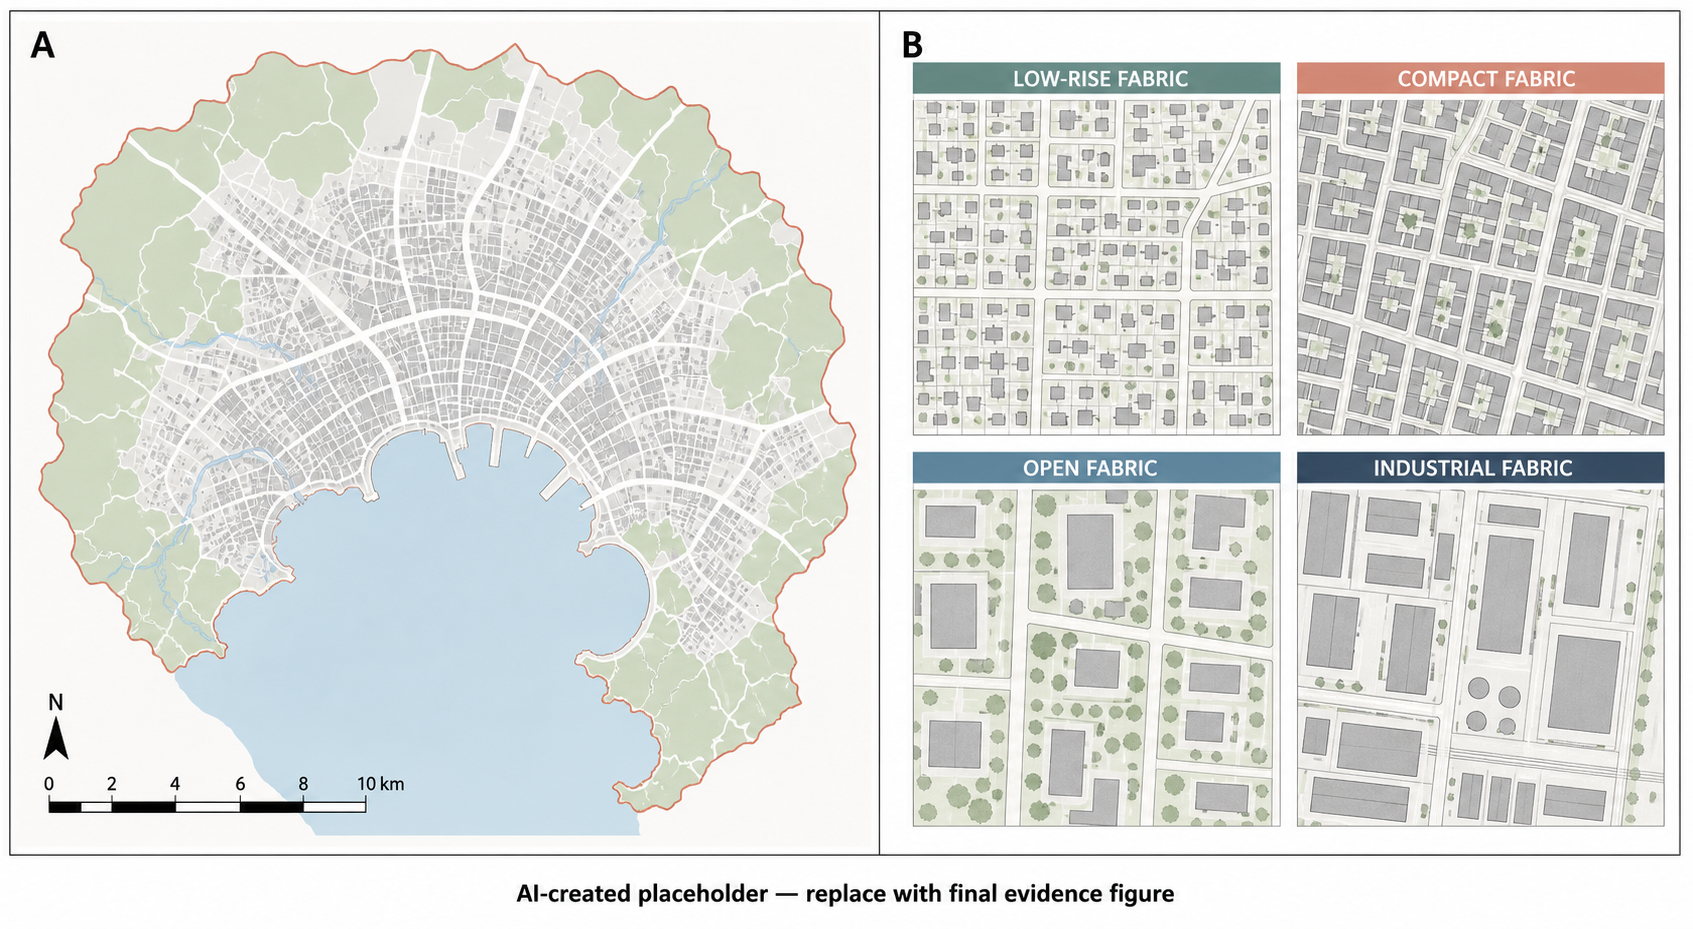
\includegraphics[width=\textwidth]{fig_1_study_area_evidence.png}
    \caption{Study-area evidence map for the Izmir functional urban region,
    showing the retained weak-label classes, summer LST response, and
    representative urban-fabric context.}
    \label{fig:study-area}
\end{figure*}

\subsection{Local morphology and surface model}

The local surface model was warped and clipped to the FUR at 5 m resolution. The accepted
working file is
\path{data/02_interim/rasters/izmir_fua_dsm5m_epsg5253.tif}. Pixels below
$-10$ m were excluded as a water/void guardrail during aggregation. Because the
surface contains terrain, buildings, vegetation, and infrastructure, we use the
terms surface-model elevation range and surface-model standard deviation, not measured building
height. Independent floor-count fields from the local building database were
converted to transparent height, floor-area-ratio, and built-volume proxies
using 3.2 m per above-ground floor. These are also named proxies throughout.

Building footprints and road centrelines from the local Akilli Sehir database
were clipped to the same boundary, yielding 356,866 buildings and 85,654 road
features. Exact footprint intersection produced coverage, density, area
heterogeneity, Gini, compactness, perimeter density, and open-space
fragmentation. Street features include exact road density, endpoint-derived
intersection and dead-end measures, degree and orientation metrics, and
road-buffer frontage continuity. Endpoint topology and frontage are not called
true graph centrality or cadastral frontage.

\subsection{Remote sensing, vegetation, coast, and functional context}

Sentinel-2 summer 2025 composites provide NDVI, NDWI, and NDBI at a 20 m working
resolution. Dynamic World summer 2025 probabilities and ESA WorldCover 2021
shares represent semantic land cover. Landsat 8/9 summer observations from
2021--2025 provide a 30 m median LST response and observation count. LST was
excluded from morphology predictors to prevent outcome leakage.

The ETH global canopy-height product supplies 10 m height and uncertainty
layers for 2020. The accepted export masks 255-valued artefacts and uses explicit
NoData. Aggregated variables include canopy cover above 2, 5, and 10 m, p95
height, and a volume proxy per hectare. Coast distance was computed from a
shoreline layer whose missing CRS metadata was assigned EPSG:5253 after
coordinate-range inspection; this assumption is preserved as a provenance
caveat.

OSM polygons, lines, and points provide proxy functional context, including
industrial/port, commercial, institutional, green/open, blue/water, transport,
military/quarry, and construction/brownfield flags. OSM is not official zoning
or an imar plan. Green-space supply for the 2SFCA uses OSM park and garden
polygons, while 2024 neighbourhood population is dasymetrically allocated to
cells in proportion to residential floor-area proxy. Table~\ref{tab:data_inventory}
records the analysis-ready sources and their roles.

\begin{table*}[htbp]
\centering
\footnotesize
\caption{Analysis-ready data inventory and provenance.}
\label{tab:data_inventory}
\resizebox{\textwidth}{!}{%
\begin{tabular}{lllll}
\toprule
Dataset & Date/period & Resolution & Role & Analysis path \\
\midrule
Study frame & Current operational boundary & vector & Izmir FUR and grid & data/02\_interim/study\_area\_fua.gpkg \\
Local surface model & local archive & 5 m & surface elevation/roughness & data/02\_interim/rasters/izmir\_fua\_dsm5m\_epsg5253.tif \\
Buildings and roads & local Akilli Sehir snapshot & vector & morphometrics/network & data/02\_interim/akilli\_sehir\_fua.gpkg \\
Global LCZ & RUB latest at extraction & 100 m working & weak labels & data/02\_interim/rasters/izmir\_fua\_lcz\_weak\_epsg5253\_100m.tif \\
Sentinel-2 & summer 2025 & 20 m working & NDVI/NDWI/NDBI & data/02\_interim/rasters/izmir\_fua\_sentinel2\_summer\_2025\_indices\_epsg5253\_20m.tif \\
Landsat 8/9 & summer 2021-2025 & 30 m & LST response & data/02\_interim/rasters/izmir\_fua\_landsat\_summer\_2021\_2025\_lst\_epsg5253\_30m.tif \\
Dynamic World & summer 2025 & 20 m working & land-cover probabilities & data/02\_interim/rasters/izmir\_fua\_dynamic\_world\_summer\_2025\_probabilities\_epsg5253\_20m.tif \\
ESA WorldCover & 2021 & 10 m & land-cover shares & data/02\_interim/rasters/izmir\_fua\_worldcover\_2021\_epsg5253\_10m.tif \\
ETH canopy height & 2020 & 10 m & vegetation height/volume proxies & data/02\_interim/rasters/izmir\_fua\_eth\_global\_canopy\_height\_2020\_clean\_epsg5253\_10m.tif \\
OSM + 2024 population & current extract / 2024 & vector + grid & 2SFCA supply/demand & data/03\_processed/grid\_green\_space\_2sfca.gpkg \\
\bottomrule
\end{tabular}%
}
\begin{minipage}{0.96\textwidth}\vspace{2pt}\scriptsize Note: All analysis layers use EPSG:5253 after harmonization. Source licences and surface-model redistribution permission must be confirmed before public release.\end{minipage}
\end{table*}



\subsection{LCZ weak labels and audit frame}

The latest RUB global LCZ image collection available at extraction was
downloaded through Google Earth Engine, clipped, warped to a 100 m working
raster, and aggregated to the 250 m grid. A weak label is the class with the
largest within-cell support; confidence is its support share. Labels are
available for 16,233 cells. At a 0.70 majority threshold, 6,585 cells are mixed.
Mixed cells are retained as transition or uncertainty candidates, not treated
as automatic errors.

The exploratory model subset was fixed before model comparison: built LCZ
classes 1--10, confidence at least 0.60, and at least 100 observations per
class. This retained 5,339 cells in LCZ 3, 6, 8, and 9. A separate 569-cell
manual-audit sample spans 40 weak-LCZ-by-built-intensity strata and is spatially
balanced. It is accompanied by an allowed-label codebook, required source and
review fields, and a three-pass priority queue. All 569 rows are now complete
and passed the audit schema gate, with 382 high-, 143 medium-, and 28 low-quality
rows; 16 edge cases carry reject flags. The audit therefore supports a bounded
descriptive validation, but its primary four-class modeling population is a
small high-quality subset and should not be read as a complete local subtype
census. Table~\ref{tab:analysis_frame} reports the current analysis status.

\begin{table}[!htbp]
\centering
\footnotesize
\caption{Analysis frame, labels, and current evidence status.}
\label{tab:analysis_frame}
\resizebox{\textwidth}{!}{%
\begin{tabular}{lrl}
\toprule
Quantity & Value & Interpretation \\
\midrule
FUR-intersecting 250 m grid units & 16,506 & Full analysis frame \\
Eligible core units & 15,801 & Boundary-coverage screen \\
Units with weak LCZ label & 16,233 & Global product aggregated to grid \\
Mixed units at 0.70 & 6,585 & Transition/uncertain units \\
Four-class analysis rows & 5,339 & LCZ 3/6/8/9, confidence >=0.60 \\
Manual audit sample & 569 & 40 LCZ-by-intensity strata \\
Completed manual audits & 569 & 382 high, 143 medium, 28 low; 16 edge rejects \\
Model matrix & 374 fields & v8, zero join losses \\
\bottomrule
\end{tabular}%
}
\end{table}



    \section{Methods}\label{sec:methodology}

\subsection{Analytical design and estimands}

The primary estimand is out-of-sample discrimination of four
high-confidence global LCZ weak labels from local climate-morphology features.
The analysis distinguishes transferable predictive signal from agreement with
local audited subtypes. Secondary estimands are (i) the
incremental predictive contribution of feature families, (ii) the paired
contribution of network 2SFCA thresholds, (iii) leave-district transfer, and
(iv) descriptive association between the weak classes, morphology, and summer
LST. Audited LCZ-like local subtype prediction is
assessed descriptively on the completed audit, but remains limited by the
small high-quality subset and the absence of a trained deep model.

The workflow is summarized in Figure~\ref{fig:workflow}. Data transformations,
model settings, and reported results are archived with the public analysis
package. Neural components are outside the present analysis and are clearly separated from the completed
tabular analysis.

\begin{figure}[!htbp]
    \centering
    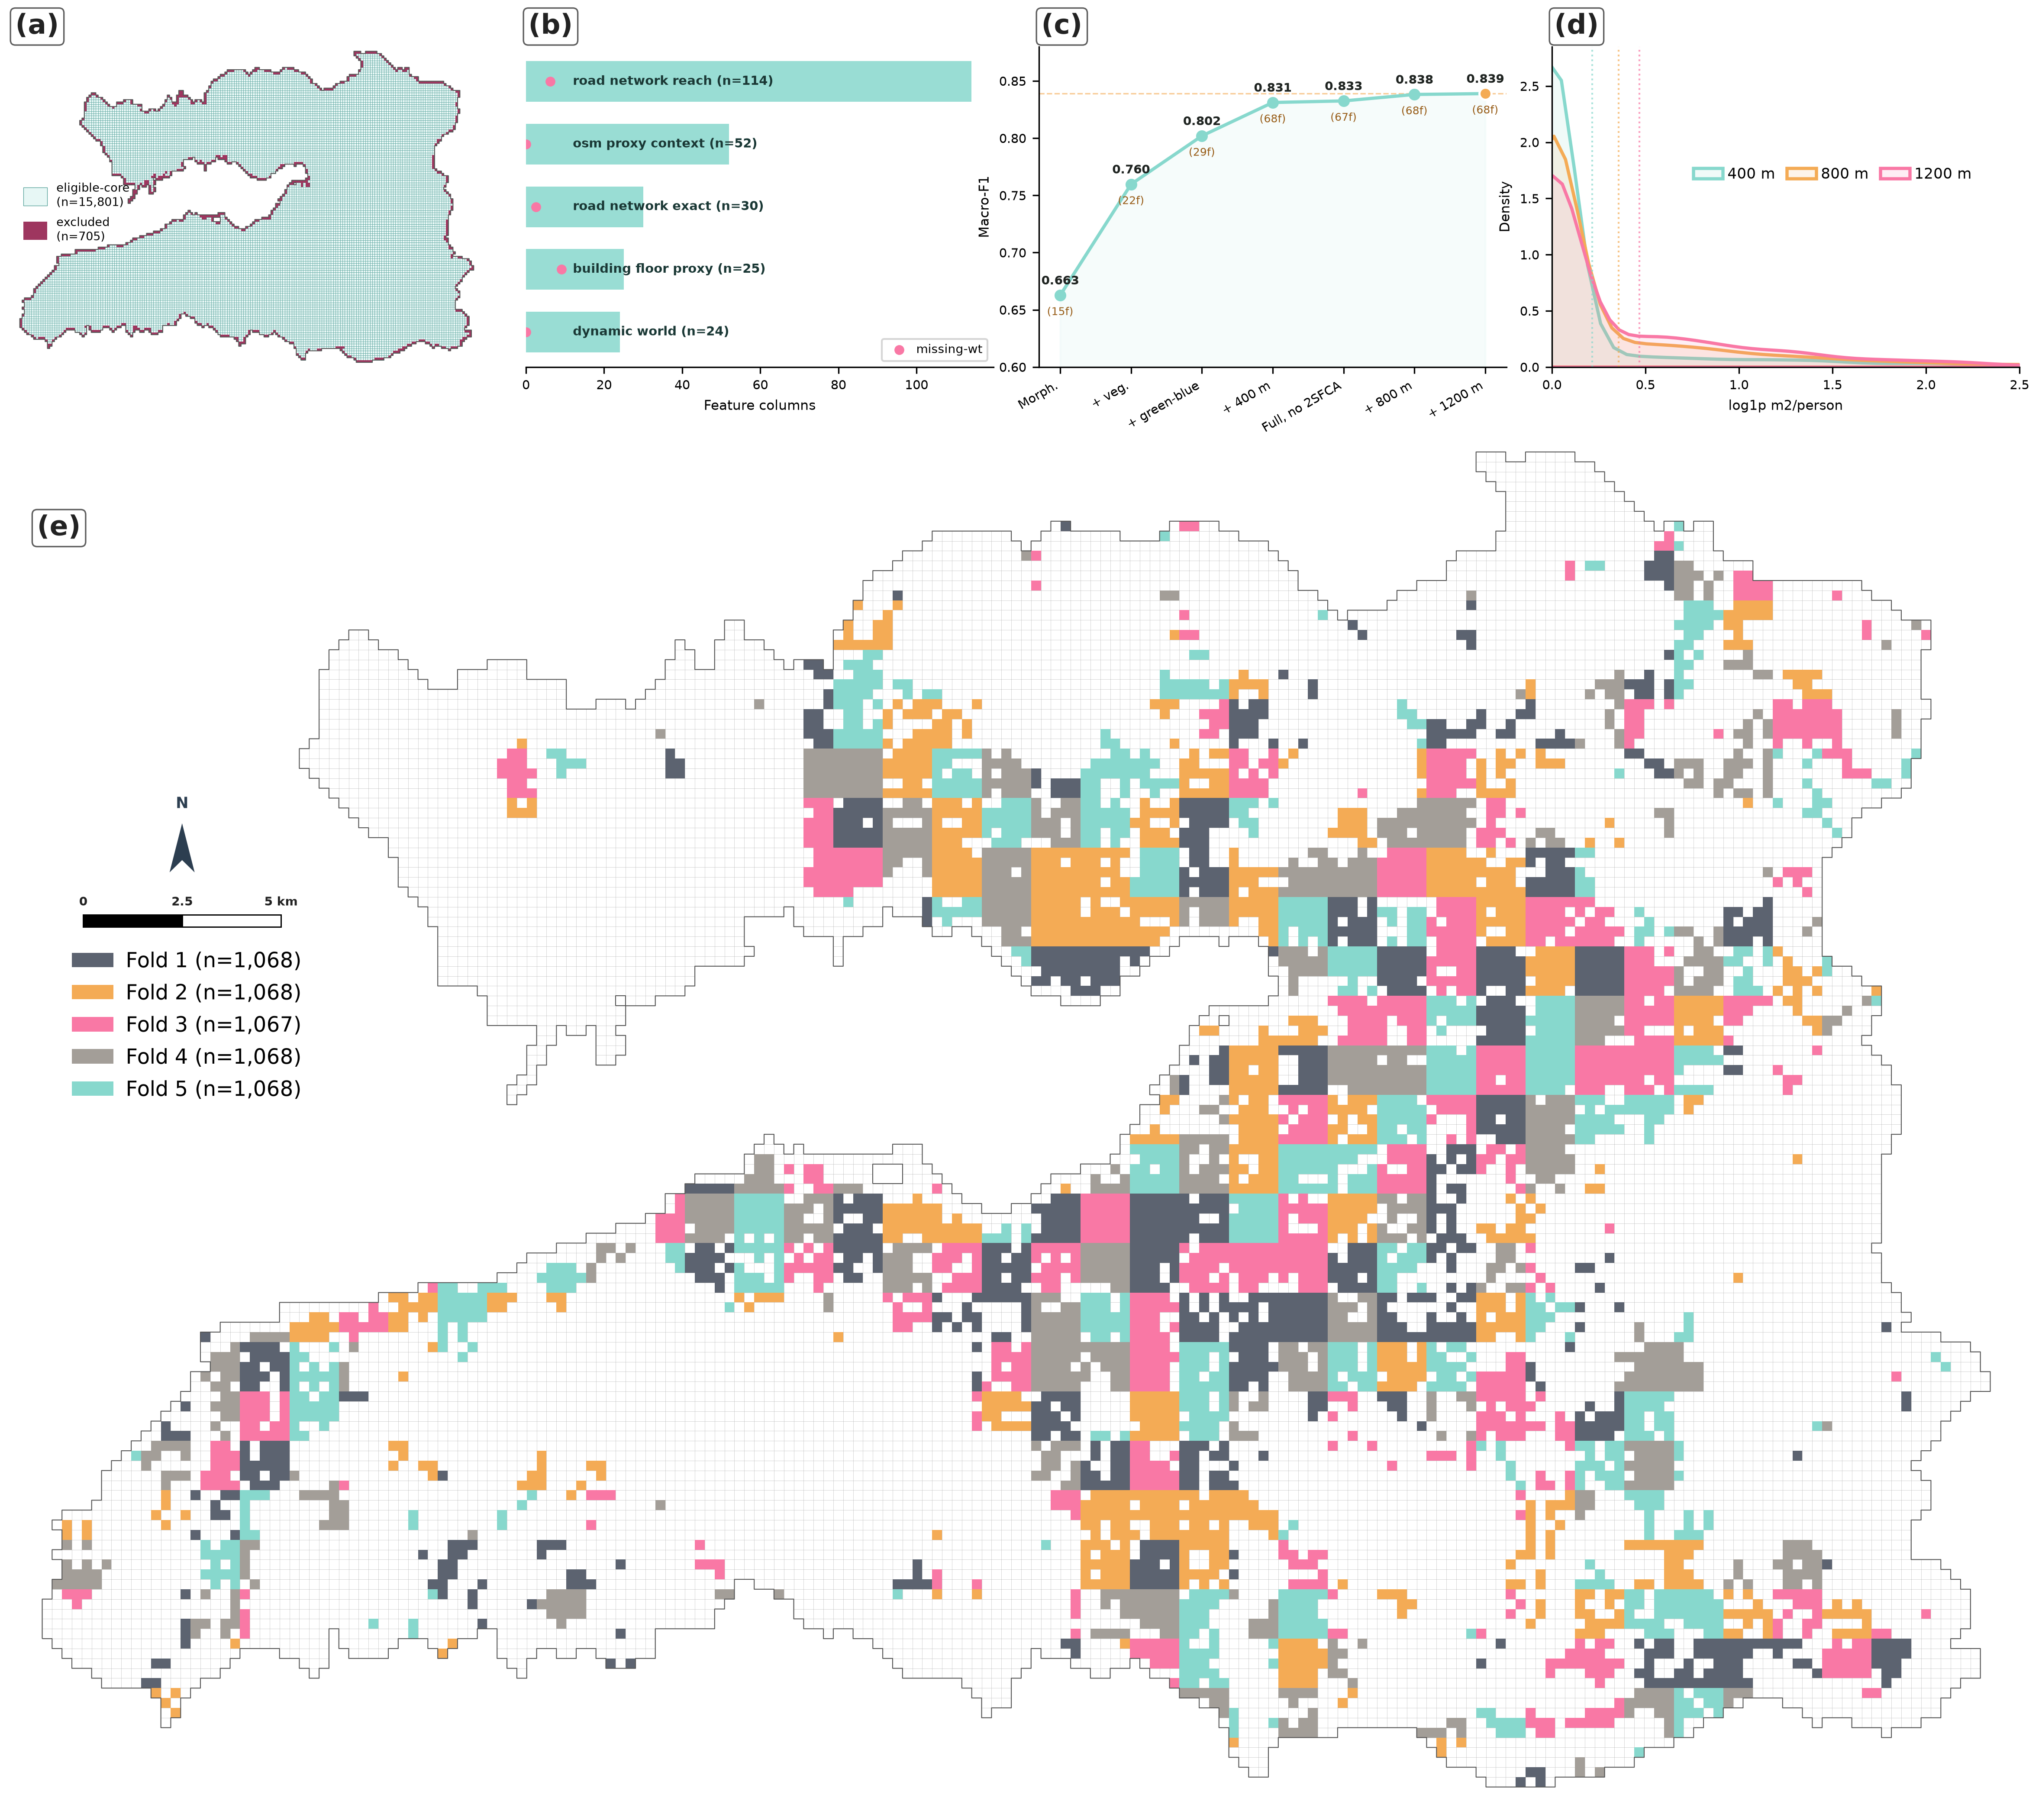
\includegraphics[width=\textwidth]{fig_2_methodology_workflow.png}
    \caption{Completed evidence workflow and confirmatory status gate. Network
    accessibility is represented by network-cost 2SFCA, whereas the legacy
    Euclidean road-context fields are supplementary only.}
    \label{fig:workflow}
\end{figure}

\subsection{Grid construction and feature engineering}

The primary grid unit is 250 m. Raster variables were summarized using valid
pixels only; vector variables were aggregated by exact intersection where
semantically appropriate. Predictor fields were screened to remove identifiers,
row/column indices, district names, weak-label quality variables, LST response
variables, and valid-pixel counts. Missingness was interpreted before
imputation: building and floor variables are structurally absent in units
without buildings, and orientation or endpoint metrics are structurally absent
without road support. The modelling pipeline uses fold-specific median
imputation rather than global imputation.

The v8 matrix contains 374 fields, of which 294 were candidate numeric
predictors after target and quality-control exclusions. At absolute correlation
$r\geq0.95$, 490 pairs formed 40 connected groups. The first baselines therefore
use representative variables and family-level ablations rather than all
available fields. Table~\ref{tab:feature_families} lists the eight interpretive
families. LST is response-only; OSM semantic context is a proxy; height,
frontage, and endpoint fields remain explicitly qualified.

\begin{table*}[htbp]
\centering
\footnotesize
\caption{Feature families used in the evidence-grounded baseline.}
\label{tab:feature_families}
\resizebox{\textwidth}{!}{%
\begin{tabular}{lll}
\toprule
Family & Representative variables & Primary role \\
\midrule
2D morphology & coverage, density, compactness, fragmentation & urban fabric \\
3D/surface model & surface-model SD/range, floor-height proxies & surface roughness/vertical intensity \\
Vegetation & canopy cover, p95 height, volume, NDVI & 3D green structure \\
Green-blue/coast & NDWI, water/tree shares, coast distance & climate context \\
Street network & road/intersection/dead-end density, entropy & connectivity proxy \\
Street interface & continuity, gap, open-buffer share & frontage proxy \\
Green access & network-cost 2SFCA at 400/800/1200 m & competition-adjusted access \\
Semantic context & Dynamic World, WorldCover, OSM shares & proxy land-use context \\
\bottomrule
\end{tabular}%
}
\begin{minipage}{0.96\textwidth}\vspace{2pt}\scriptsize Note: LST and label-quality fields were excluded from predictors. OSM, floor count, frontage, and endpoint topology remain explicitly named proxies.\end{minipage}
\end{table*}



\subsection{Network-cost green-space 2SFCA}

Green-space context is defined by supply, demand, and shortest-path cost rather
than by a circular buffer. OSM park and garden polygon area provides supply
$S_j$. The 2024 neighbourhood population is allocated to 250 m units as demand
$P_i$ in proportion to residential floor-area proxy. Municipal road
centrelines are planarized after excluding explicitly coded motorways. Origins
and green-space access points are snapped to this network; their snap distances
are included in generalized distance $d_{ij}$.

For threshold $d_0$, step 1 calculates the supply--demand ratio

\begin{equation}
R_j = \frac{S_j}{\sum_{i:d_{ij}\leq d_0} P_i},
\end{equation}

and step 2 assigns each unit

\begin{equation}
A_i = \sum_{j:d_{ij}\leq d_0} R_j.
\end{equation}

The preregistered primary threshold is 800 m, with 400 and 1,200 m sensitivity
thresholds. Raw square metres per person are retained for description;
$\log(1+A_i)$ enters the model because of the long upper tail. This is an OSM
and municipal-road-network accessibility proxy, not a pedestrian routing
product, official public-green inventory, or measure of park quality.

To audit supply geography, the 2023-modified IZBB north/south park-maintenance
inventory was normalized by district and neighbourhood. It has no coordinates
or public-access field and is limited to branch responsibility. We therefore
compare log counts and log areas by district and use leave-one-district-out
correlation ranges. Name matching is used only as a quality check.

\subsection{Weak-label definition and audit sampling}

For unit $i$, the weak label is

\begin{equation}
l_i^{weak}=\arg\max_c A_{ic},
\end{equation}

where $A_{ic}$ is class-$c$ area or probability support. Weak confidence is

\begin{equation}
conf_i^{weak}=\max_c(A_{ic}/A_i).
\end{equation}

The manual-audit sample was allocated across weak class and preliminary
built-intensity strata. If $N_h$ is the size of stratum $h$, $N$ is the frame,
$n$ is the target sample, and $n_{min}$ protects rare strata, the initial
allocation follows

\begin{equation}
n_h=\max\{n_{min},\mathrm{round}(nN_h/N)\},
\end{equation}

with certainty selection where a stratum is smaller than its target. Spatial
balance prevents the sample from collapsing into common central fabrics. The
priority queue changes review order only; it does not change the sampling
frame, inclusion weights, or validation role.

\subsection{Baseline models and additive ablations}

Four tabular learners were evaluated as complementary baselines. Random Forest
used 300 trees, minimum leaf size 2, square-root feature sampling, and
balanced-subsample class weights. Extra Trees used the same tree count and leaf
size with balanced class weights. XGBoost used 300 histogram-based trees,
maximum depth 6, and learning rate 0.1 with fold-specific balanced sample
weights. LightGBM used 300 trees, learning rate 0.1, balanced class weights,
and gain-based feature importance. A majority classifier provided a floor.
Random seed 42 controls fold construction; fold-specific seeds control models.

Four nested recipes isolate information families. Recipe A contains 15 2D/3D
morphology variables. Recipe B adds seven vegetation-structure variables.
Recipe C adds seven coastal and green-blue variables. Recipe D adds remote
spectral and semantic variables, OSM proxy context, exact street-network
metrics, street-interface proxies, and one 2SFCA field, for 68 predictors. The
2SFCA experiment compares recipe D with the accessibility field omitted and
with otherwise identical 400, 800, or 1,200 m fields. Because semantic remote
sensing may overlap with the global LCZ weak-label production process, the
nested results are interpreted as discrimination evidence, not independent
causal contribution.

\subsection{Spatial validation and transfer testing}

The main validation uses five-fold StratifiedGroupKFold. Spatial groups are
5-by-5-grid-unit blocks, nominally 1.25 km, and no block appears in both training and
test data within a fold. Median imputation is fit only to each training fold.
Metrics are accuracy, balanced accuracy, weighted F1, macro-F1, and per-class
precision, recall, and F1. Out-of-fold probabilities provide the uncertainty
map.

A separate leave-one-district-out (LODO) transfer test evaluates the LightGBM recipe
D, with Random Forest as a comparison baseline. Districts with at least 100
eligible observations were held out one at a time, yielding 11 tests and 5,279
test predictions. Because several held-out
districts do not contain all four classes, LODO macro-F1 is calculated over
classes present in that district and is reported alongside balanced accuracy.
This is a harder transfer test, not a replacement for spatial blocks.

\subsection{Ablation, explainability, and uncertainty}

Additive ablations are compared on the same folds. For each 2SFCA threshold,
fold-level macro-F1 and balanced-accuracy differences are paired with the same
model without 2SFCA. Gain-based LightGBM importance is averaged across the five
primary fits. This importance is useful for screening but can be biased toward
correlated or high-cardinality predictors; it is not interpreted as a causal
effect. Out-of-fold maximum probability is mapped as a first uncertainty
indicator. A fuller multimodal study would additionally require calibrated
probabilities, SHAP for tabular components, and spatial attribution for neural
branches.

\subsection{Climate-response validation}

LST is never a morphology predictor. For the 5,339-unit analysis subset, we
report class-specific medians and interquartile ranges, a Kruskal--Wallis test,
and epsilon-squared effect size

\begin{equation}
\epsilon^2=\frac{H-k+1}{n-k},
\end{equation}

where $H$ is the Kruskal statistic, $k$ is the number of classes, and $n$ is the
valid sample. Spearman correlations connect selected morphology, vegetation,
network, coast, and 2SFCA variables to LST. These are bivariate descriptive
associations. They do not estimate cooling causality or air-temperature
exposure.

\subsection{Confirmatory CLIMORFA architecture and stopping rule}

The confirmatory architecture has three branches: (i) raster chips for
Sentinel, land-cover probabilities, and the 5 m surface model; (ii) multichannel
figure-ground chips for buildings, streets, open space, vegetation, and height
coding; and (iii) tabular morphometric, vegetation, coast, network, and 2SFCA
features. Each branch creates an embedding $e_b$. Late fusion concatenates
embeddings,

\begin{equation}
z_i=[e_{r,i};e_{g,i};e_{t,i}],
\end{equation}

or uses learned gates $\alpha_b$,

\begin{equation}
z_i=\sum_{b\in\{r,g,t\}}\alpha_b W_b e_{b,i}.
\end{equation}

Mandatory ablations remove the surface model, vegetation, network, figure-ground, and remote
semantic inputs. Integrated Gradients, Grad-CAM or occlusion, and tabular SHAP
are required. These analyses cannot enter the
abstract, headline tables, or conclusion as a deep-model performance claim
until the branches are trained and evaluated on an audited spatial-validation
design. This paper therefore reports an evidence-grounded tabular
baseline and bounded audit validation, not CLIMORFA deep-model performance.

    \section{Results}\label{sec:results}

\subsection{Data readiness and label frame}

The v8 integration completed without row loss: all 16,506 grid units are
present and 374 fields are available. Remote-sensing, surface-model, and climate-response
families have low missingness, whereas building, floor, frontage, and network
families show the expected structural absence where the relevant
objects. The highest family-average missing share is 36.3\% for floor proxies;
surface-model missingness averages 0.7\% and canopy height 1.8\%. Figure~\ref{fig:data-readiness}
contrasts feature-family missingness with the four-class analysis population.
composition. LCZ 6 is the largest class (1,842), followed by LCZ 8 (1,317), LCZ
9 (1,099), and LCZ 3 (1,081).

The manual audit is complete: all 569 sampled units passed the schema gate, comprising
382 high-, 143 medium-, and 28 low-quality rows, with 16 edge-case reject flags.
Weak-versus-audit agreement and bounded audited model comparisons are therefore
available, although the primary four-class comparison is limited to 96
high-quality units and retains substantial class-space compression.

\begin{figure}[H]
    \centering
    \includegraphics[width=\textwidth]{fig_3_data_readiness.png}
    \caption{Data readiness and audit design. Panels (a--c) show representative
    250 m grid, LST, imagery, and feature evidence; (d) maps the complete
    569-unit audit sample by review pass; and (e) compares audit-quality flags
    with priority scores. Missingness can be structural and is not automatically
    an error.}
    \label{fig:data-readiness}
\end{figure}

\subsection{Weak-class climate-morphology profiles}

The retained weak classes were morphologically distinct (Table~\ref{tab:class_profiles};
Figure~\ref{fig:class-profiles}). LCZ 3 had the highest median building coverage
(0.380) and floor-height proxy (11.10 m). LCZ 8 combined intermediate coverage
(0.191) and height (8.33 m) with the highest summer median LST, 46.09~$^{\circ}$C.
LCZ 6 and LCZ 9 were much more open: median coverage was 0.024 and 0.001,
respectively, and median LST was 43.01 and 43.27~$^{\circ}$C. LCZ 6 and LCZ 9
also had higher median NDVI (0.331 and 0.353) than LCZ 3 and LCZ 8 (0.137 and
0.132).

\begin{table*}[htbp]
\centering
\footnotesize
\caption{Median climate-morphology profiles of the four retained weak-label classes.}
\label{tab:class_profiles}
\resizebox{\textwidth}{!}{%
\begin{tabular}{lrrrrrrrr}
\toprule
Class & n & LST & Coverage (\%) & Height proxy (m) & Surface-model SD (m) & Canopy (\%) & NDVI & 2SFCA log1p \\
\midrule
LCZ 3 & 1,081 & 44.85 & 38.0 & 11.10 & 7.26 & 100.0 & 0.137 & 0.567 \\
LCZ 6 & 1,842 & 43.01 & 2.4 & 6.37 & 9.30 & 91.3 & 0.331 & 0.000 \\
LCZ 8 & 1,317 & 46.09 & 19.1 & 8.33 & 5.17 & 87.7 & 0.132 & 0.217 \\
LCZ 9 & 1,099 & 43.27 & 0.1 & 3.20 & 9.87 & 80.7 & 0.353 & 0.000 \\
\bottomrule
\end{tabular}%
}
\begin{minipage}{0.96\textwidth}\vspace{2pt}\scriptsize Note: Descriptive weak-label profiles; they are not manually audited local subtypes.\end{minipage}
\end{table*}



\begin{figure}[H]
    \centering
    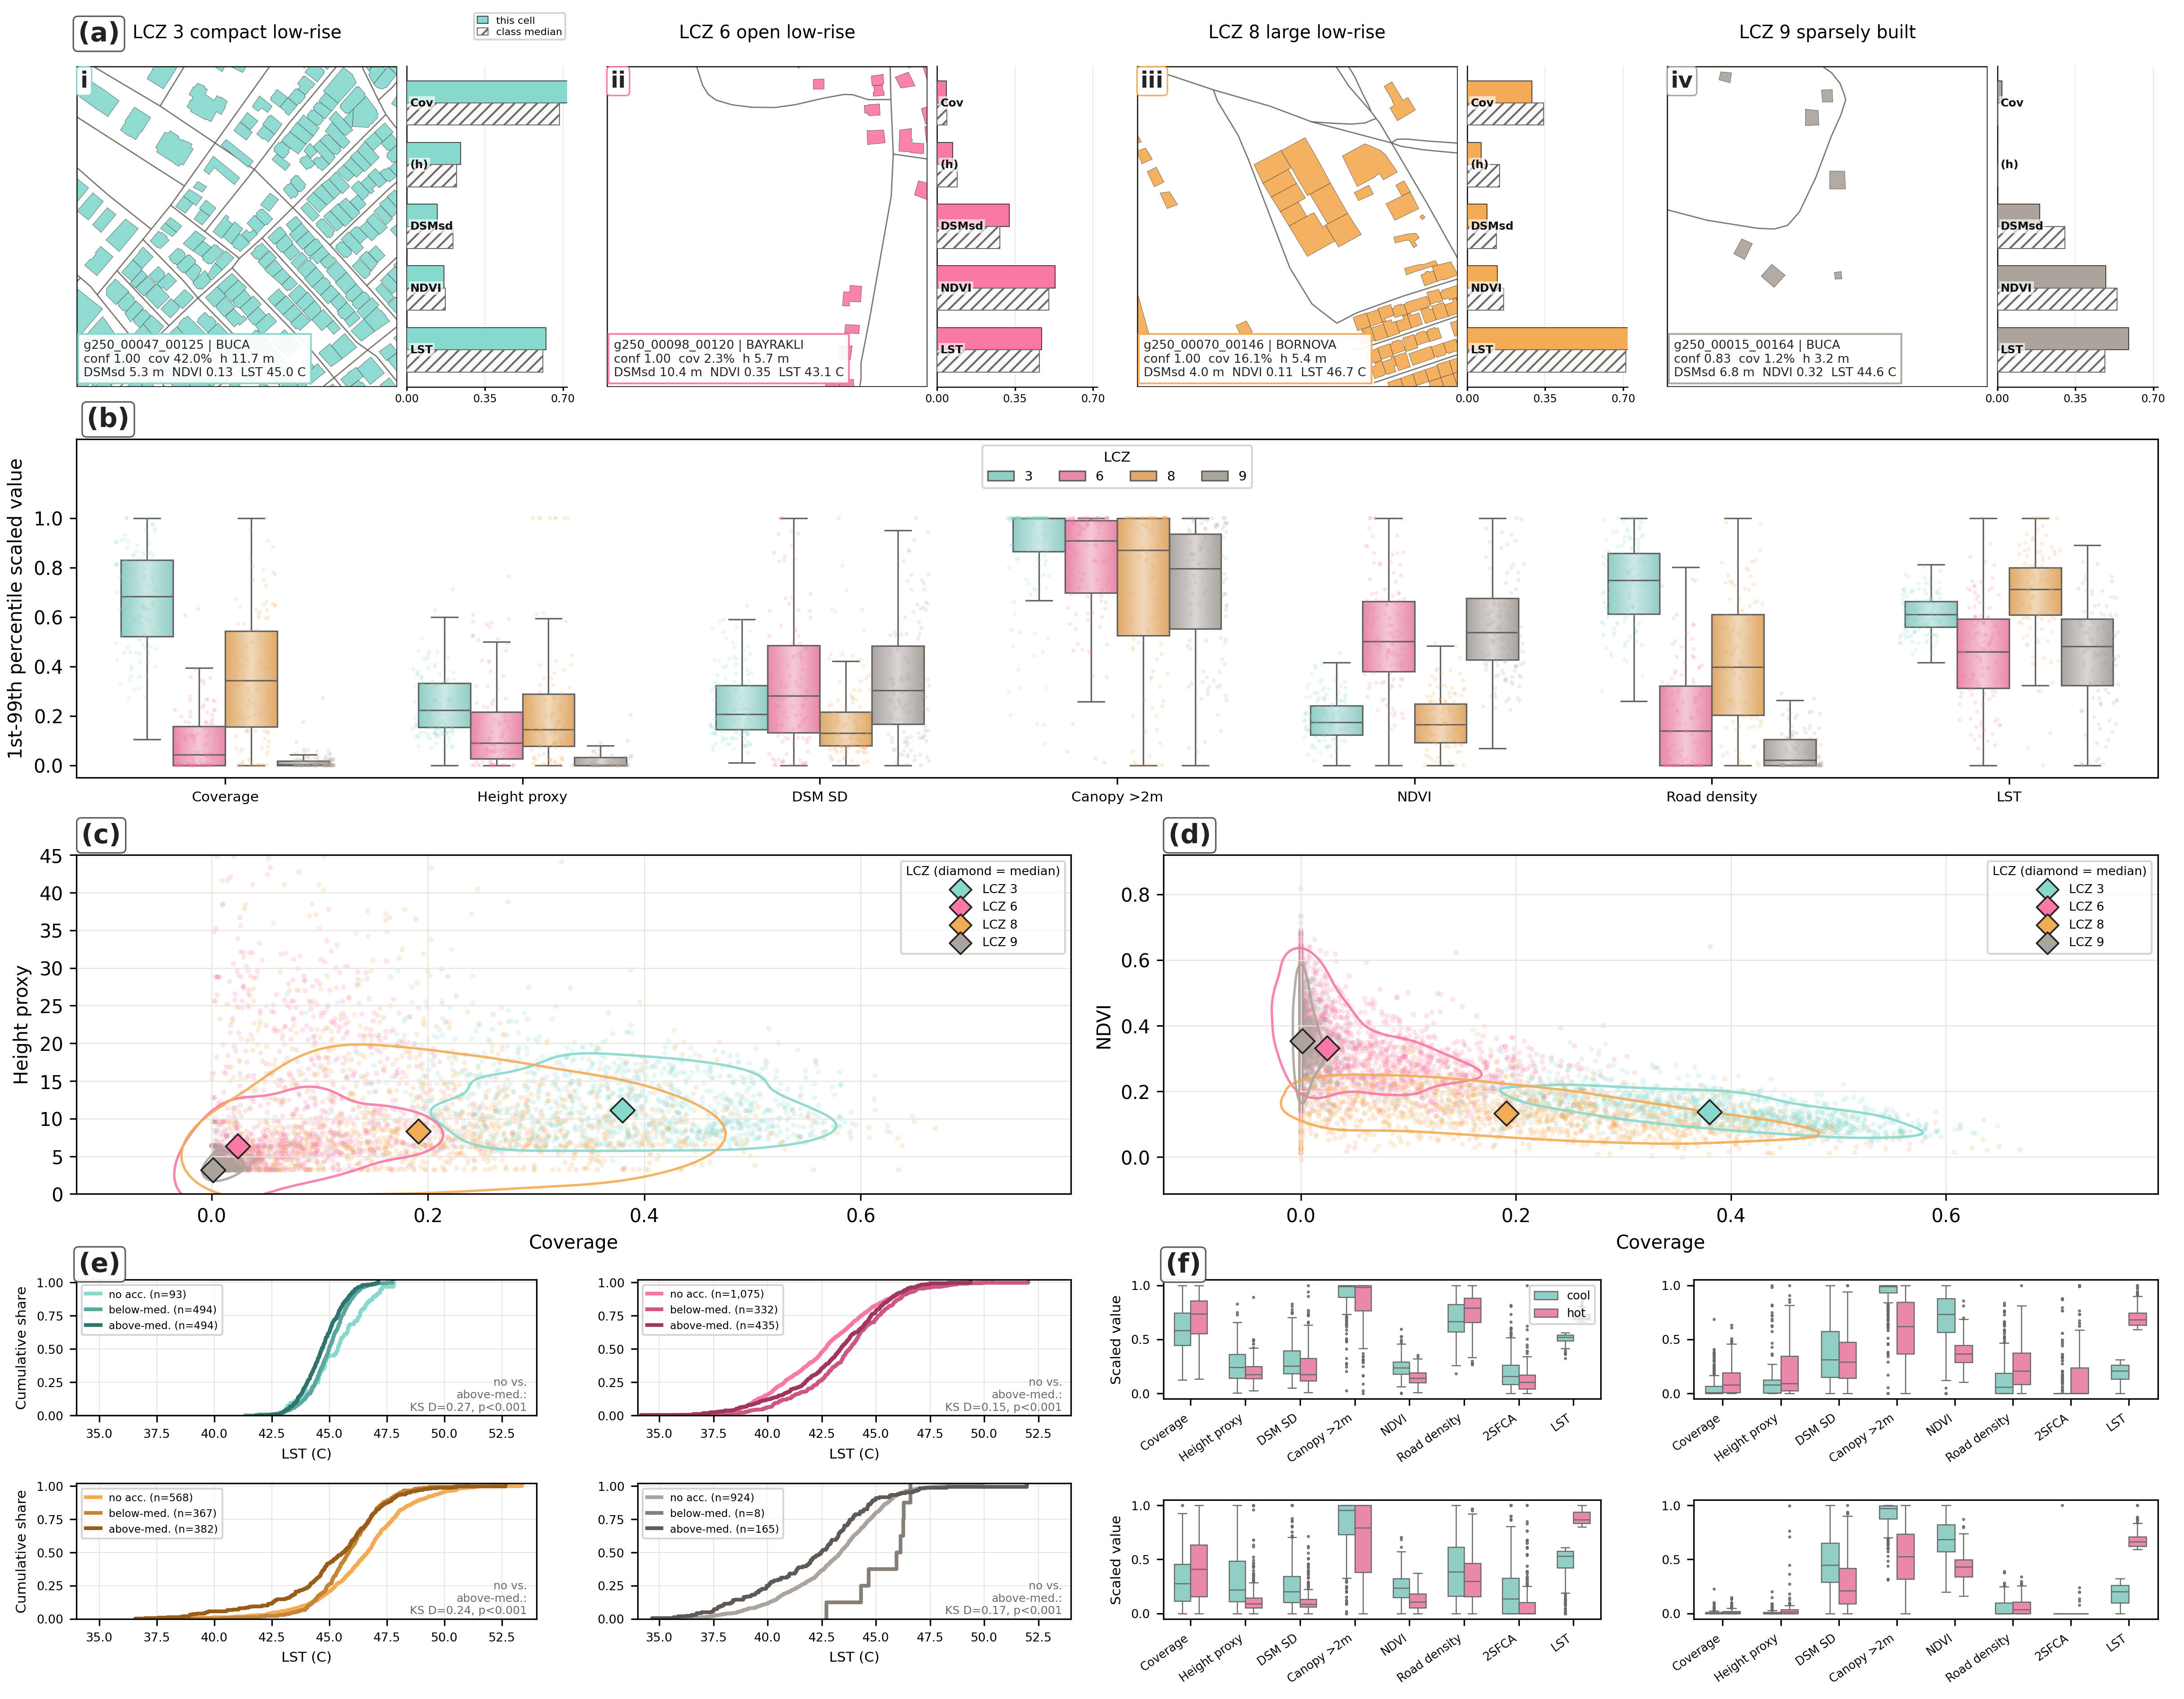
\includegraphics[width=0.78\textwidth]{fig_4_class_profiles.png}
    \caption{Weak-class profiles. Colour expresses each class median standardized
    across the four classes; annotations are raw medians. Structural missingness
means the displayed height-proxy medians use available building-bearing units.}
    \label{fig:class-profiles}
\end{figure}

These contrasts are consistent with the broad semantics of the global labels,
but they remain weak-label profiles rather than a substitute for the audited
local class space. In particular, canopy
cover above 2 m is high in all four classes because the ETH surface-height
product and threshold capture vegetation pixels wherever present; it should not
be read as public green-space share. Likewise, road density is a geometric
network measure rather than walkability.

\subsection{Spatial-block baseline performance and ablation}

The majority classifier produced macro-F1 0.128. LightGBM morphology-only
macro-F1 was 0.663; adding vegetation raised it to 0.760, and green-blue
context raised it to 0.802. The full recipe without 2SFCA reached 0.833, while
the preregistered 800 m recipe reached 0.838 for LightGBM, 0.835 for XGBoost,
0.829 for Random Forest, and 0.819 for Extra Trees (Figure~\ref{fig:baseline-performance};
Table~\ref{tab:baseline_performance}). The LightGBM standard deviation at the
primary recipe was 0.012. The 1,200 m alternative was marginally higher for
LightGBM (0.839), so the 800 m result is retained as the prespecified primary
rather than selected post hoc.

\begin{figure}[!htbp]
    \centering
    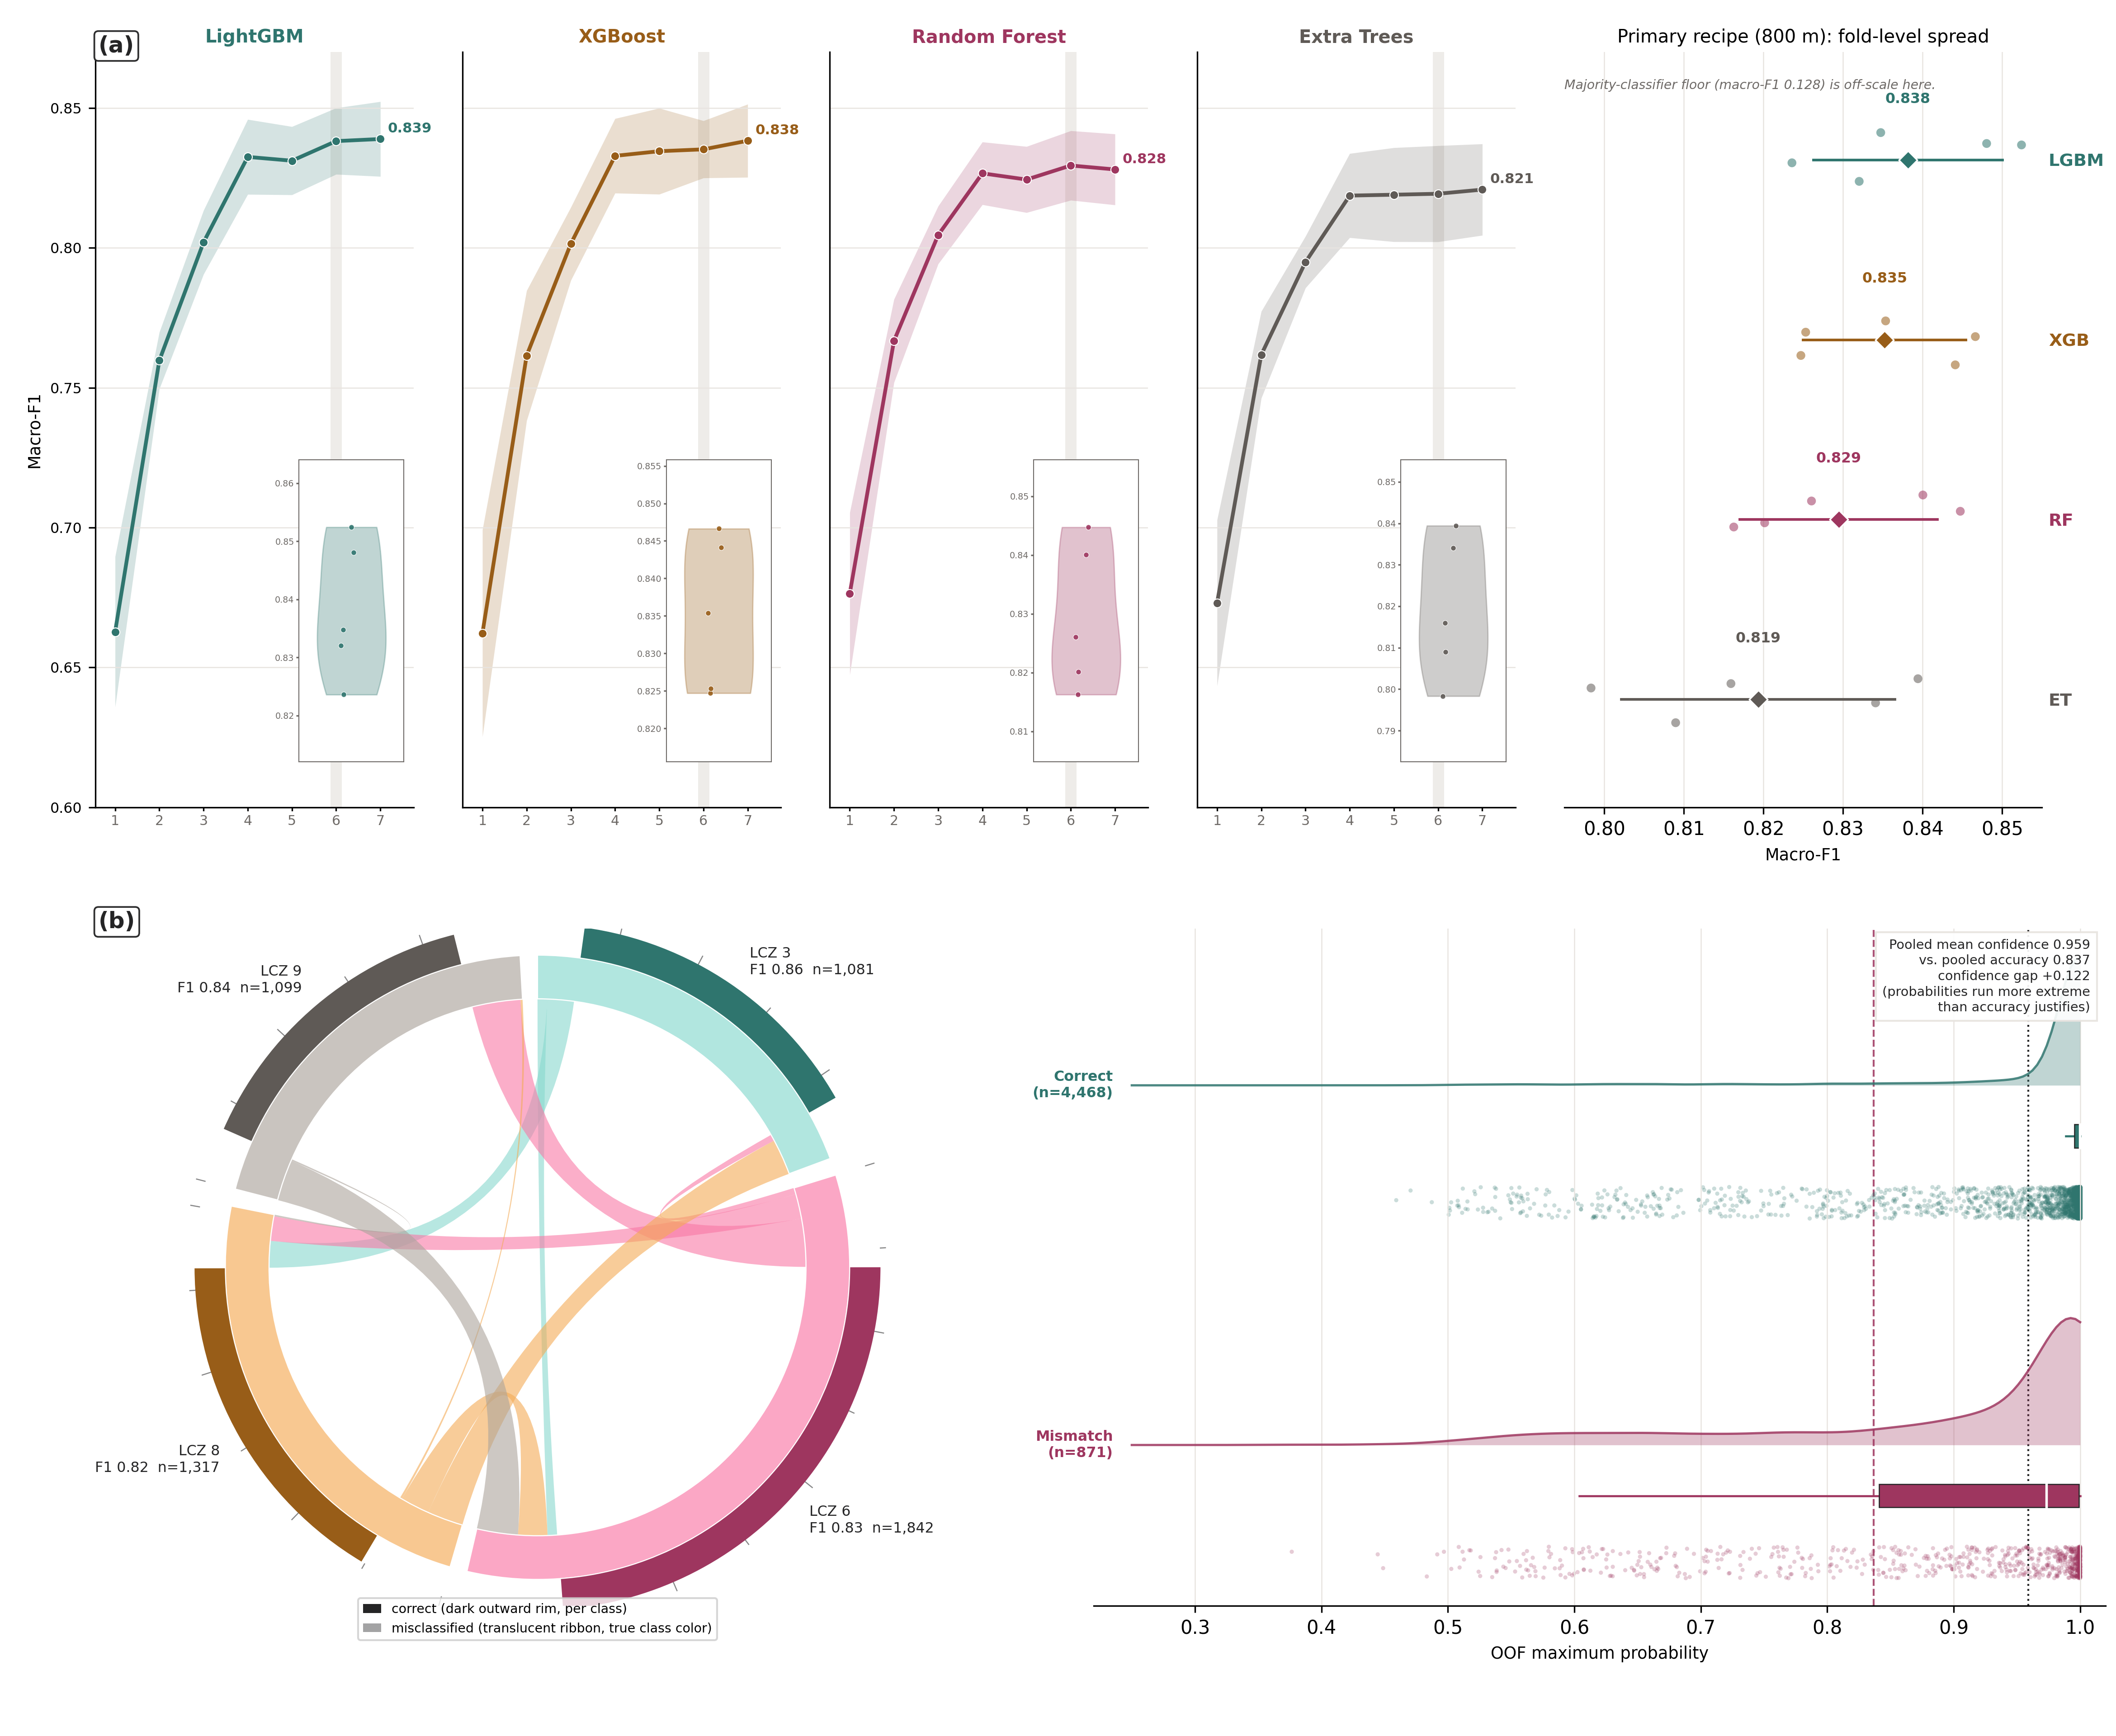
\includegraphics[width=0.92\textwidth]{fig_5_baseline_performance.png}
    \caption{Mean macro-F1 under five spatial block folds for four tabular
    learners. Recipes are additive and the shaded position marks the
    prespecified 800 m recipe. All targets are global weak labels.}
    \label{fig:baseline-performance}
\end{figure}

\begin{table*}[htbp]
\centering
\scriptsize
\caption{Five-fold stratified spatial-block weak-label performance.}
\label{tab:baseline_performance}
\setlength{\tabcolsep}{3pt}
\resizebox{\textwidth}{!}{%
\begin{tabular}{llrrr}
\toprule
Model & Recipe & Features & Macro-F1 (mean $\pm$ SD) & Balanced accuracy \\
\midrule
XGBoost & Morphology & 15 & 0.662 $\pm$ 0.037 & 0.678 \\
LightGBM & Morphology & 15 & 0.663 $\pm$ 0.027 & 0.669 \\
Extra Trees & Morphology & 15 & 0.673 $\pm$ 0.030 & 0.705 \\
Random Forest & Morphology & 15 & 0.676 $\pm$ 0.029 & 0.688 \\
LightGBM & + vegetation & 22 & 0.760 $\pm$ 0.010 & 0.762 \\
XGBoost & + vegetation & 22 & 0.761 $\pm$ 0.023 & 0.766 \\
Extra Trees & + vegetation & 22 & 0.762 $\pm$ 0.016 & 0.776 \\
Random Forest & + vegetation & 22 & 0.767 $\pm$ 0.015 & 0.772 \\
Extra Trees & + green-blue & 29 & 0.795 $\pm$ 0.009 & 0.803 \\
XGBoost & + green-blue & 29 & 0.801 $\pm$ 0.013 & 0.805 \\
LightGBM & + green-blue & 29 & 0.802 $\pm$ 0.011 & 0.804 \\
Random Forest & + green-blue & 29 & 0.805 $\pm$ 0.010 & 0.808 \\
Extra Trees & Full, no 2SFCA & 67 & 0.819 $\pm$ 0.015 & 0.824 \\
Random Forest & Full, no 2SFCA & 67 & 0.827 $\pm$ 0.011 & 0.827 \\
LightGBM & Full, no 2SFCA & 67 & 0.833 $\pm$ 0.013 & 0.834 \\
XGBoost & Full, no 2SFCA & 67 & 0.833 $\pm$ 0.013 & 0.836 \\
Extra Trees & Full + 400 m & 68 & 0.819 $\pm$ 0.017 & 0.824 \\
Random Forest & Full + 400 m & 68 & 0.824 $\pm$ 0.012 & 0.825 \\
LightGBM & Full + 400 m & 68 & 0.831 $\pm$ 0.012 & 0.832 \\
XGBoost & Full + 400 m & 68 & 0.835 $\pm$ 0.015 & 0.837 \\
Extra Trees & Full + 800 m & 68 & 0.819 $\pm$ 0.017 & 0.825 \\
Random Forest & Full + 800 m & 68 & 0.829 $\pm$ 0.012 & 0.830 \\
XGBoost & Full + 800 m & 68 & 0.835 $\pm$ 0.010 & 0.838 \\
LightGBM & Full + 800 m & 68 & 0.838 $\pm$ 0.012 & 0.839 \\
Extra Trees & Full + 1200 m & 68 & 0.821 $\pm$ 0.016 & 0.826 \\
Random Forest & Full + 1200 m & 68 & 0.828 $\pm$ 0.013 & 0.828 \\
XGBoost & Full + 1200 m & 68 & 0.838 $\pm$ 0.013 & 0.841 \\
LightGBM & Full + 1200 m & 68 & 0.839 $\pm$ 0.013 & 0.840 \\
\bottomrule
\end{tabular}%
}
\begin{minipage}{0.96\textwidth}\vspace{2pt}\scriptsize Note: Blocks are nominally 1.25 km (5 by 5 cells). Preprocessing is fit within each training fold. Values are mean $\pm$ standard deviation across five folds. These are exploratory weak-label diagnostics; within each recipe, models are ordered by descending macro-F1.\end{minipage}
\end{table*}


Pooled out-of-fold LightGBM F1 was 0.861 for LCZ 3, 0.833 for LCZ 6, 0.820 for
LCZ 8, and 0.839 for LCZ 9 (Table~\ref{tab:class_metrics}). The lower F1 for
LCZ 8 indicates overlap or heterogeneity around large low-rise fabrics, even
though the class has the highest LST profile.

\begin{table}[!htbp]
\centering
\scriptsize
\caption{Pooled out-of-fold class performance for the primary 800 m recipe.}
\label{tab:class_metrics}
\resizebox{\textwidth}{!}{%
\begin{tabular}{llrrrr}
\toprule
Model & Class & Support & Precision & Recall & F1 \\
\midrule
LightGBM & LCZ 3 & 1081 & 0.852 & 0.870 & 0.861 \\
LightGBM & LCZ 6 & 1842 & 0.833 & 0.834 & 0.833 \\
LightGBM & LCZ 8 & 1317 & 0.838 & 0.803 & 0.820 \\
LightGBM & LCZ 9 & 1099 & 0.828 & 0.850 & 0.839 \\
XGBoost & LCZ 3 & 1081 & 0.850 & 0.873 & 0.862 \\
XGBoost & LCZ 6 & 1842 & 0.837 & 0.819 & 0.828 \\
XGBoost & LCZ 8 & 1317 & 0.828 & 0.800 & 0.813 \\
XGBoost & LCZ 9 & 1099 & 0.817 & 0.860 & 0.838 \\
Random Forest & LCZ 3 & 1081 & 0.843 & 0.886 & 0.864 \\
Random Forest & LCZ 6 & 1842 & 0.813 & 0.828 & 0.821 \\
Random Forest & LCZ 8 & 1317 & 0.840 & 0.778 & 0.808 \\
Random Forest & LCZ 9 & 1099 & 0.823 & 0.829 & 0.826 \\
Extra Trees & LCZ 3 & 1081 & 0.819 & 0.896 & 0.856 \\
Extra Trees & LCZ 6 & 1842 & 0.822 & 0.792 & 0.807 \\
Extra Trees & LCZ 8 & 1317 & 0.834 & 0.759 & 0.795 \\
Extra Trees & LCZ 9 & 1099 & 0.792 & 0.851 & 0.820 \\
\bottomrule
\end{tabular}%
}
\end{table}


\subsection{Feature importance and out-of-fold uncertainty}

LightGBM gain importance was distributed across remote semantic, 2D form,
vegetation, climate context, 3D/surface, street-network, and green-access
families (Figure~\ref{fig:importance}). Remote semantics contributed 48.0\% of
the normalized primary-recipe importance, followed by 2D form (20.2\%),
vegetation (10.4\%), and context (8.9\%); 2SFCA contributed 1.3\%. The leading
individual variables included WorldCover built-up share, building perimeter
density, Sentinel-2 NDWI, coast distance, Dynamic World crop probability, and
NDVI. This mixture supports multi-family integration, but it also confirms that
remote semantic information may share signal with the weak LCZ target. The
importance ranking is therefore an explanation of the model, not proof of an
independent physical mechanism.

\begin{figure}[!htbp]
    \centering
    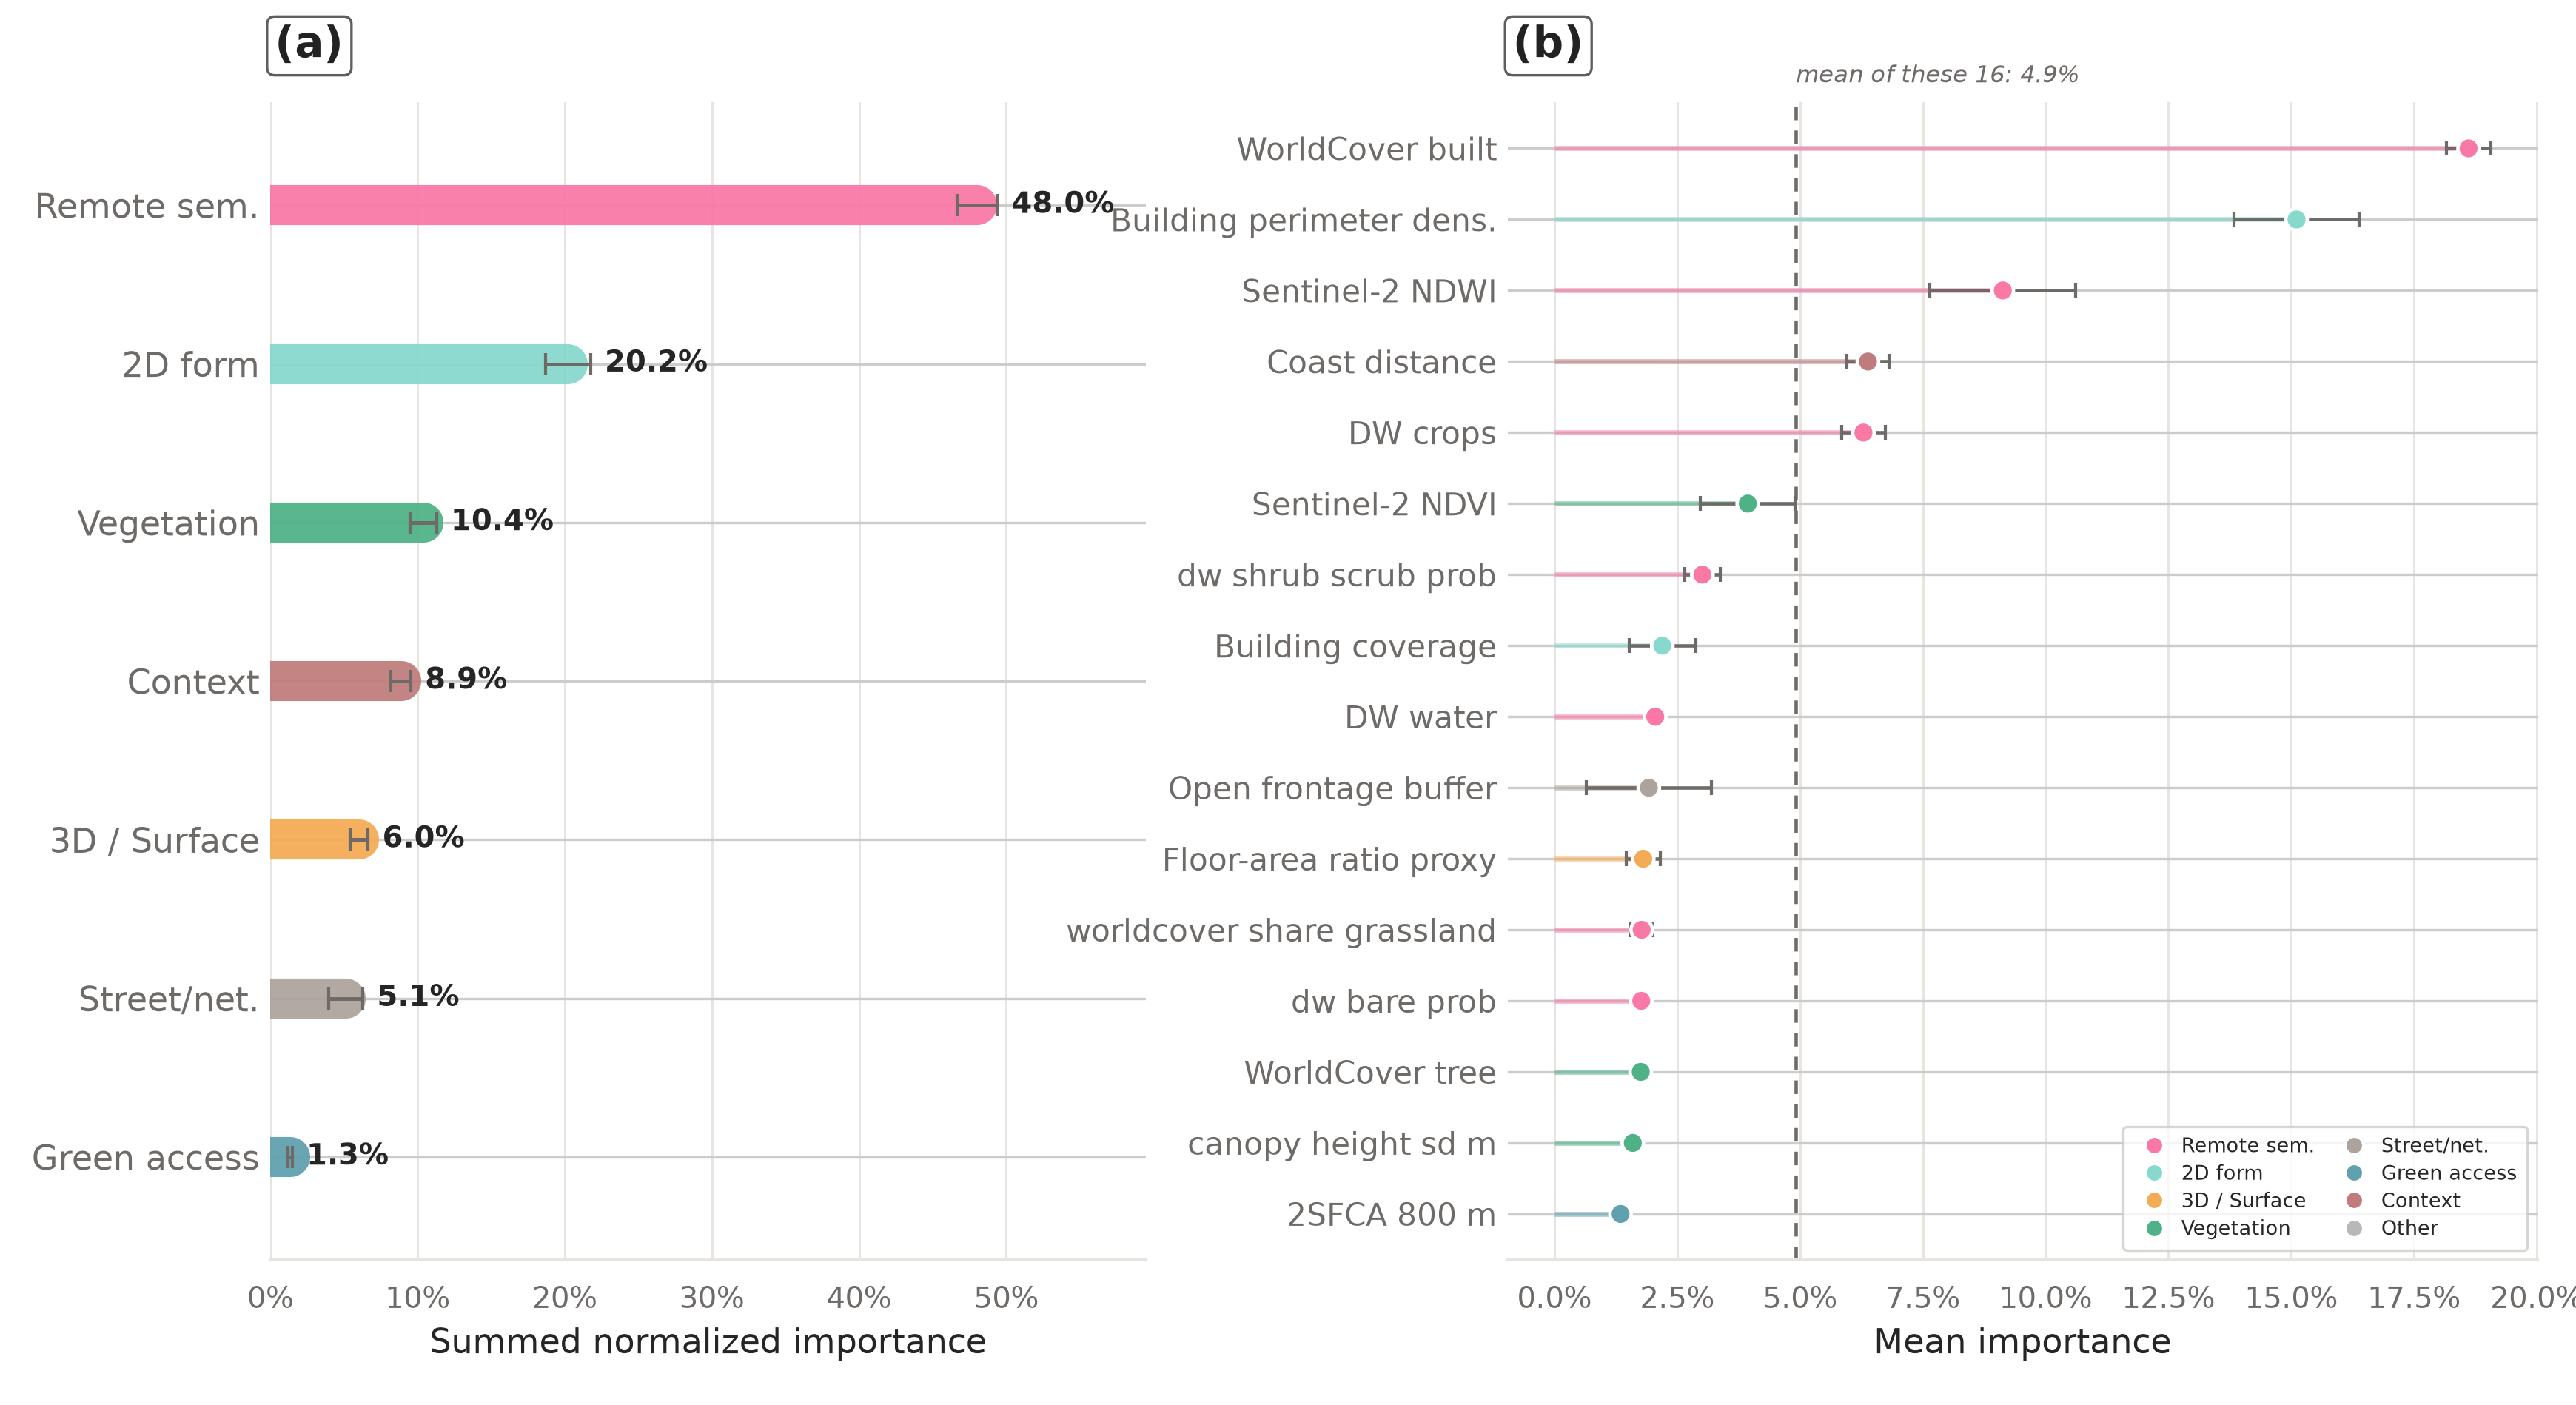
\includegraphics[width=0.88\textwidth]{fig_6_feature_importance.png}
    \caption{Mean LightGBM gain importance across the five primary 800 m folds,
    normalized within each fold. Error bars are between-fold standard deviations.}
    \label{fig:importance}
\end{figure}

The primary LightGBM mean out-of-fold maximum probability was 0.959, compared
with pooled accuracy 0.837; correct predictions numbered 4,468 and mismatches
871. Figure~\ref{fig:uncertainty} reveals spatial clusters of lower confidence
and audit-compatible/contradictory units. Probability is not calibrated
confidence, however; the warning score is used as a stability indicator rather
than a planning-risk estimate.

\begin{figure}[!htbp]
    \centering
    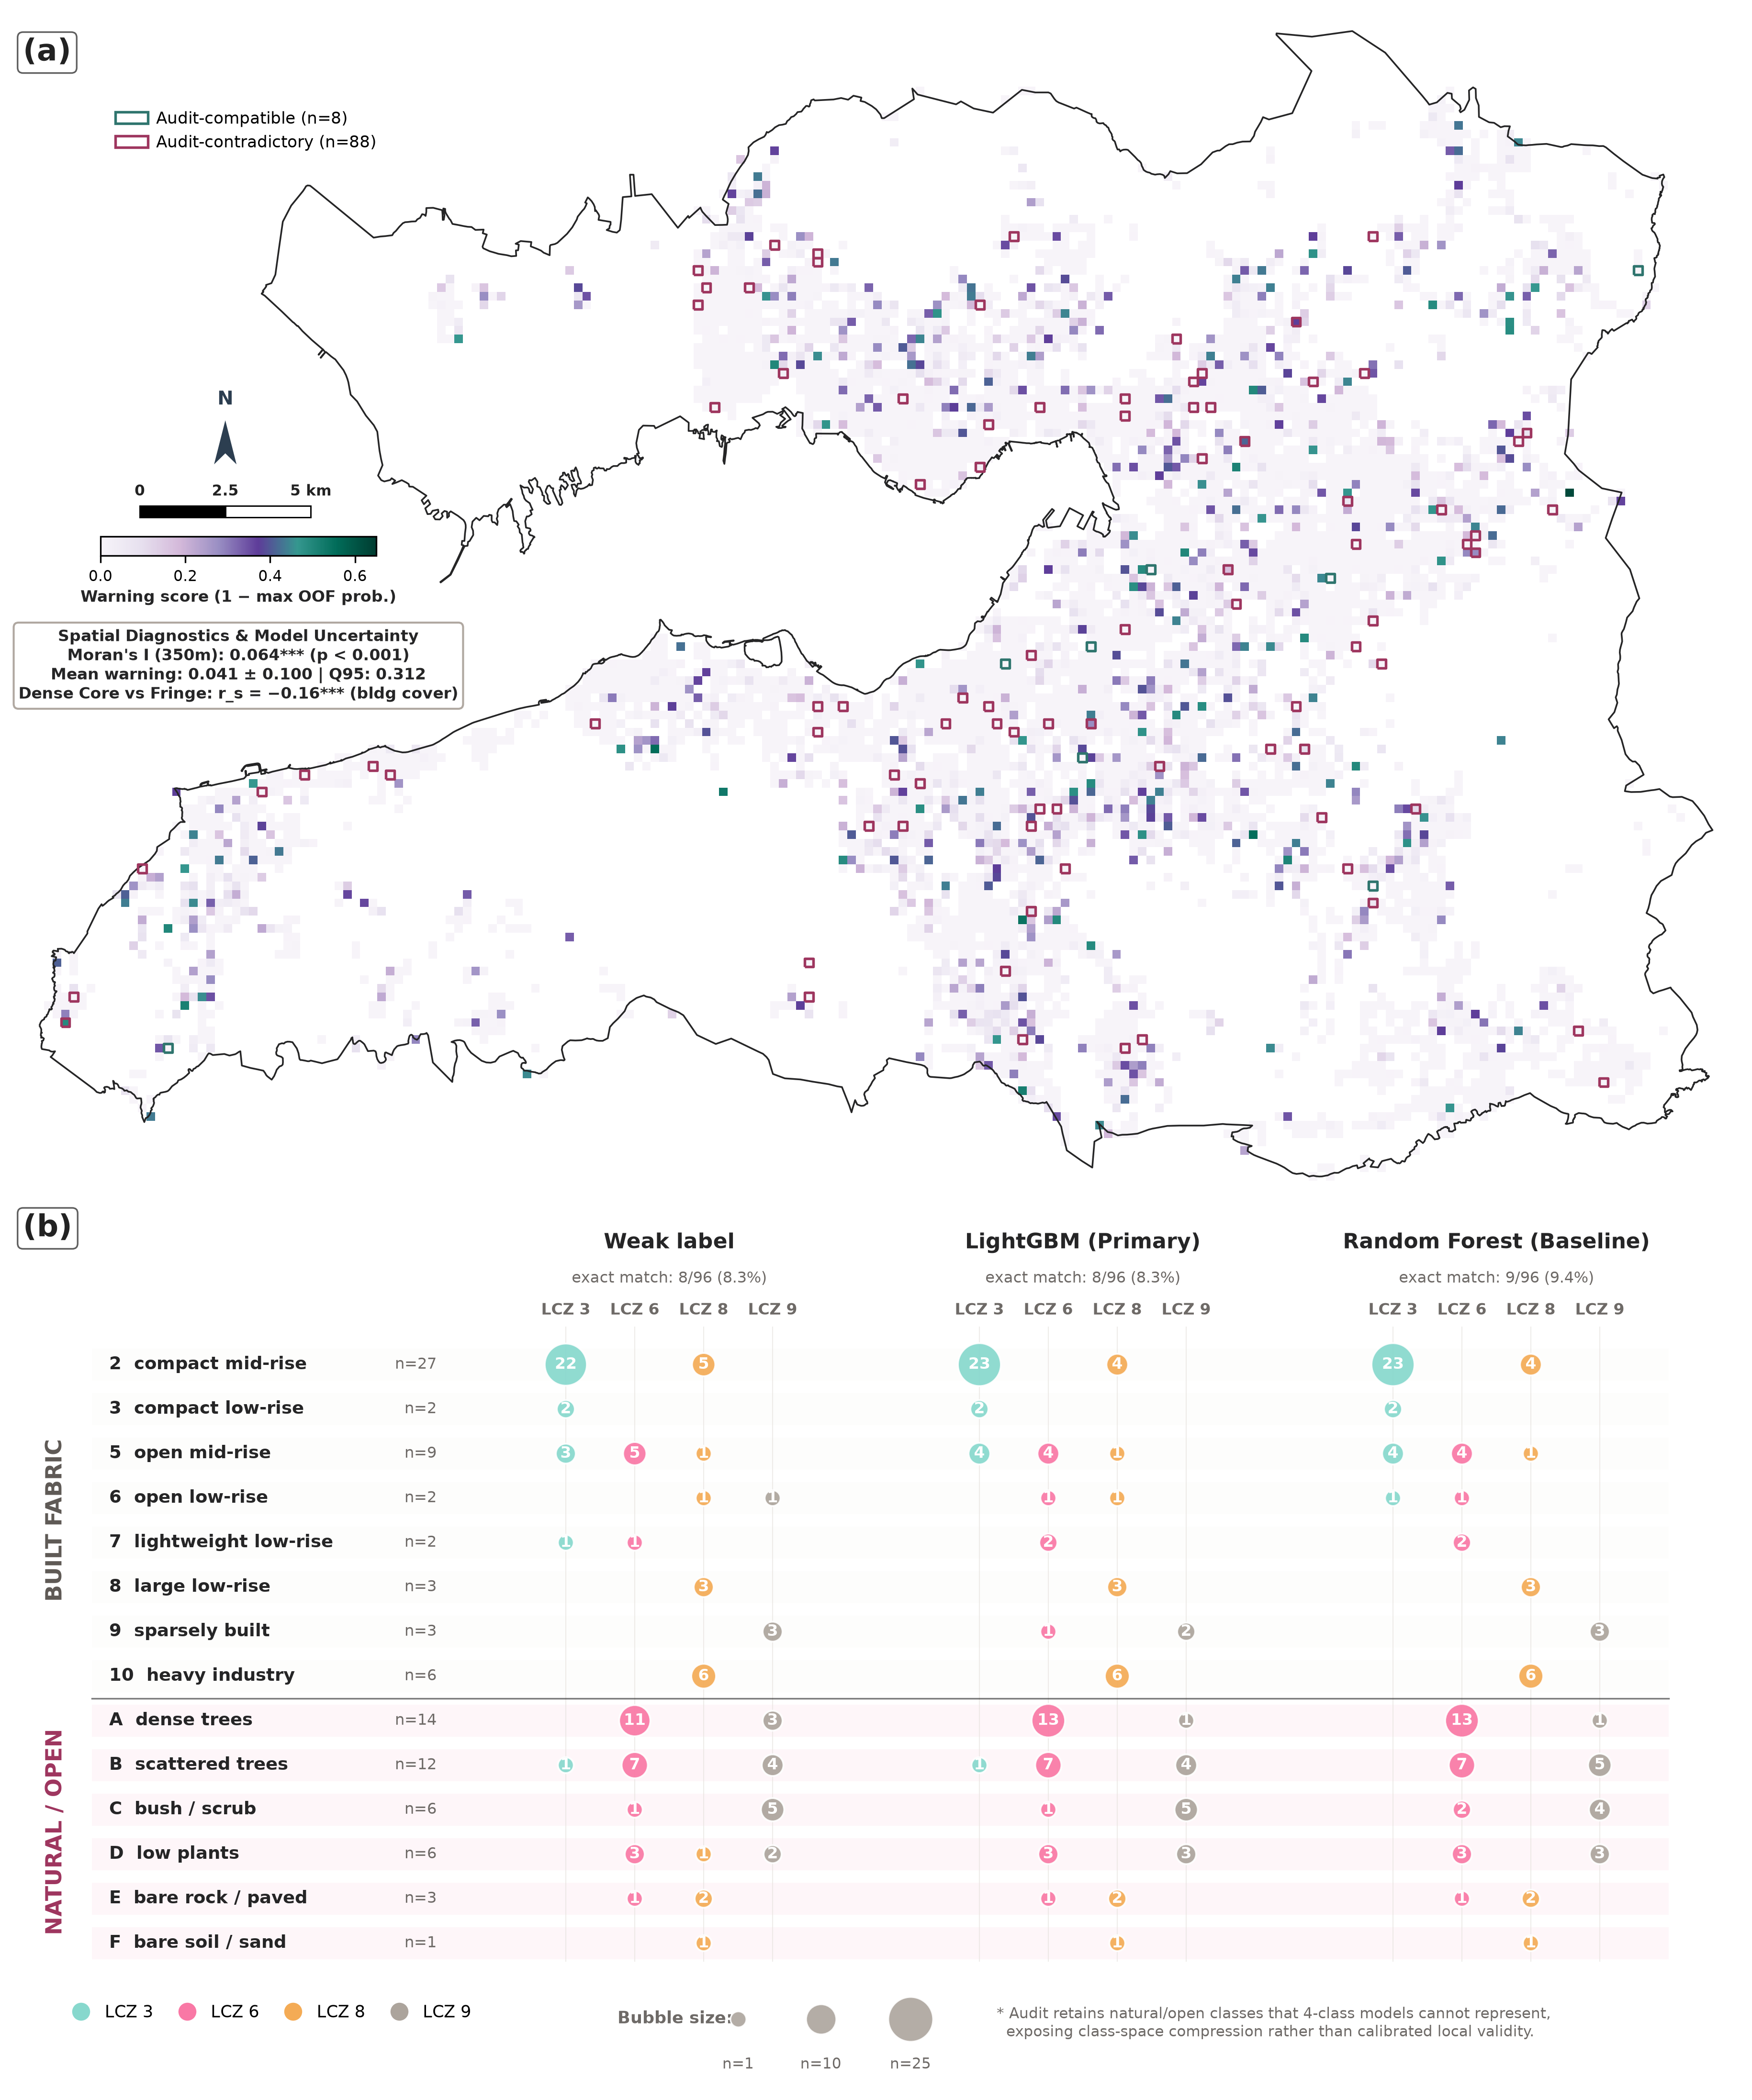
\includegraphics[width=\textwidth]{fig_7_uncertainty.png}
    \caption{Out-of-fold LightGBM uncertainty for the primary recipe. (a) Spatial
    warning score with the completed high-quality audit overlay. (b) Weak-label,
    LightGBM, and Random Forest audit crosswalks. Agreement shares are
    descriptive and the probabilities are not calibrated confidence.}
    \label{fig:uncertainty}
\end{figure}

\subsection{Network 2SFCA threshold sensitivity}

Compared with the same full model without 2SFCA, the primary 800 m field
increased mean macro-F1 by 0.0056 for LightGBM, 0.0023 for XGBoost, 0.0028 for
Random Forest, and 0.0007 for Extra Trees. The 1,200 m alternative was slightly
higher for LightGBM (0.0064 above no 2SFCA), while threshold effects varied by
model. Figure~\ref{fig:2sfca-sensitivity} shows why these thresholds are treated
as sensitivity parameters: access geography changes with catchment radius, and
larger radii add both supply and competing demand. The 800 m threshold remains
primary by design rather than by post-hoc reselection.

\begin{figure}[!htbp]
    \centering
    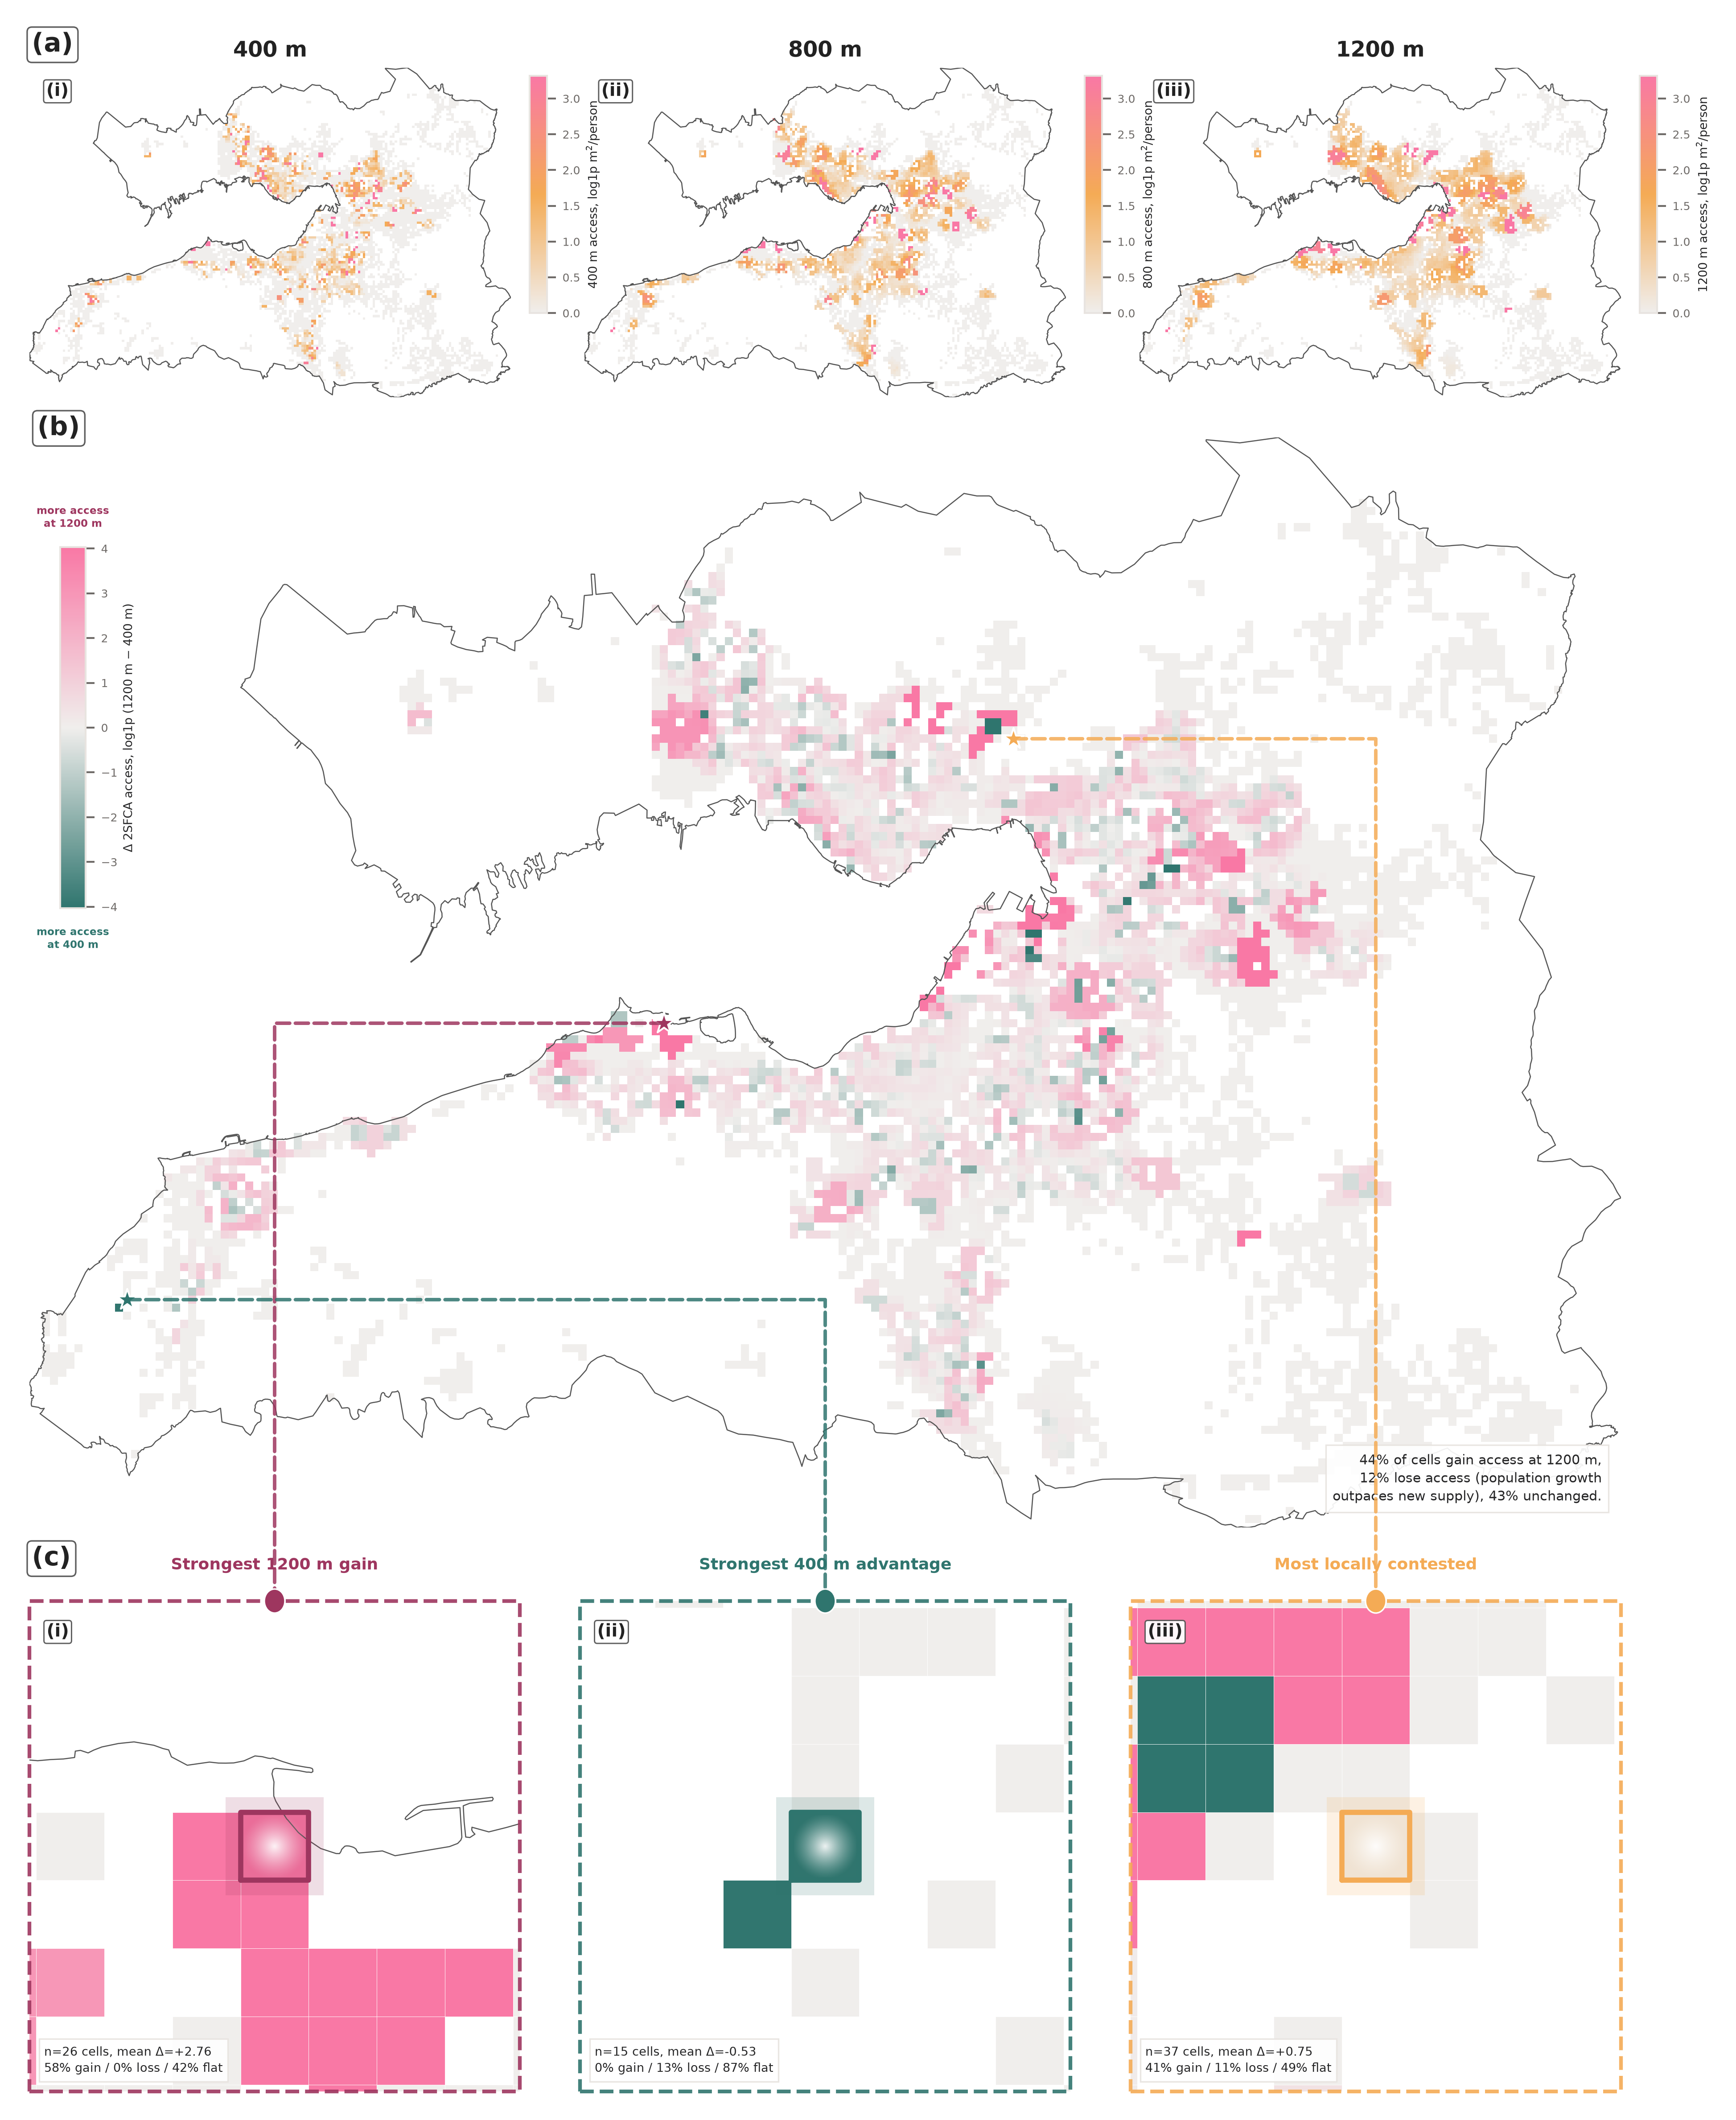
\includegraphics[width=\textwidth]{fig_8_2sfca_sensitivity.png}
    \caption{Network-cost 2SFCA scale sensitivity. (a) Access geography at
    400, 800, and 1,200 m. (b) The 1,200 m minus 400 m access difference. (c)
    Zoomed examples of strongest gain, strongest 400 m advantage, and local
    contestation. The figure is descriptive of access geography; model-score
    deltas are reported in Table~\ref{tab:2sfca}.}
    \label{fig:2sfca-sensitivity}
\end{figure}

\begin{table*}[htbp]
\centering
\footnotesize
\caption{Paired 2SFCA threshold contribution relative to the same model without 2SFCA.}
\label{tab:2sfca}
\resizebox{\textwidth}{!}{%
\begin{tabular}{llrrrr}
\toprule
Model & Threshold & Mean delta & SD & Fold wins & Range \\
\midrule
LightGBM & 400 m & -0.0014 & 0.0033 & 1/5 & [-0.0057, +0.0036] \\
LightGBM & 800 m & +0.0056 & 0.0036 & 5/5 & [+0.0017, +0.0088] \\
LightGBM & 1200 m & +0.0064 & 0.0079 & 3/5 & [-0.0021, +0.0171] \\
XGBoost & 400 m & +0.0017 & 0.0080 & 3/5 & [-0.0059, +0.0129] \\
XGBoost & 800 m & +0.0023 & 0.0067 & 3/5 & [-0.0053, +0.0106] \\
XGBoost & 1200 m & +0.0054 & 0.0061 & 4/5 & [-0.0043, +0.0110] \\
Random Forest & 400 m & -0.0022 & 0.0052 & 2/5 & [-0.0095, +0.0028] \\
Random Forest & 800 m & +0.0028 & 0.0035 & 4/5 & [-0.0030, +0.0054] \\
Random Forest & 1200 m & +0.0014 & 0.0030 & 3/5 & [-0.0021, +0.0050] \\
Extra Trees & 400 m & +0.0003 & 0.0019 & 4/5 & [-0.0028, +0.0021] \\
Extra Trees & 800 m & +0.0007 & 0.0040 & 3/5 & [-0.0058, +0.0035] \\
Extra Trees & 1200 m & +0.0021 & 0.0060 & 3/5 & [-0.0047, +0.0094] \\
\bottomrule
\end{tabular}%
}
\begin{minipage}{0.96\textwidth}\vspace{2pt}\scriptsize Note: Threshold performance is interpreted as sensitivity, not post-hoc model selection; the 800 m threshold is primary by design. Deltas are paired within the same spatial folds.\end{minipage}
\end{table*}


The municipal source audit strengthens only the macro spatial interpretation.
The official dataset contained 189 distinct park sites; 180 sites in 112 matched
FUR neighbourhoods were comparable with 644 OSM polygons across 12 districts.
Pearson correlations on log counts and areas were 0.931 and 0.910, and
leave-one-district-out ranges were 0.882--0.945 and 0.808--0.928. Rank
correlations were lower (0.747 and 0.776). Only 10.6\% of comparable official
sites had exact or strong OSM name candidates, and only 417 of 1,237 total OSM
supply polygons were named. OSM supply therefore reproduces broad district
geography but cannot be called complete or equivalent to official public green
space.

\subsection{Leave-district-out transfer}

LODO LightGBM macro-F1 averaged 0.723 across 11 districts, with a standard
deviation of 0.104 and range 0.475--0.819 (Figure~\ref{fig:lodo};
Table~\ref{tab:leave_district}). G\"uzelbah\c{c}e (0.475), Konak (0.598), and
Bal\c{c}ova (0.682) were the hardest transfers, while Kar\c{s}\i yaka (0.819),
Karaba\u{g}lar (0.807), Narl\i dere (0.794), and Bayrakl\i{} (0.775) were
stronger. Mean accuracy was 0.818 and mean balanced accuracy 0.766. The decline
from spatial-block macro-F1 0.838 to district-held-out 0.723 indicates that
within-FUR geographic transfer is materially harder than local block
interpolation.

\begin{figure}[!htbp]
    \centering
    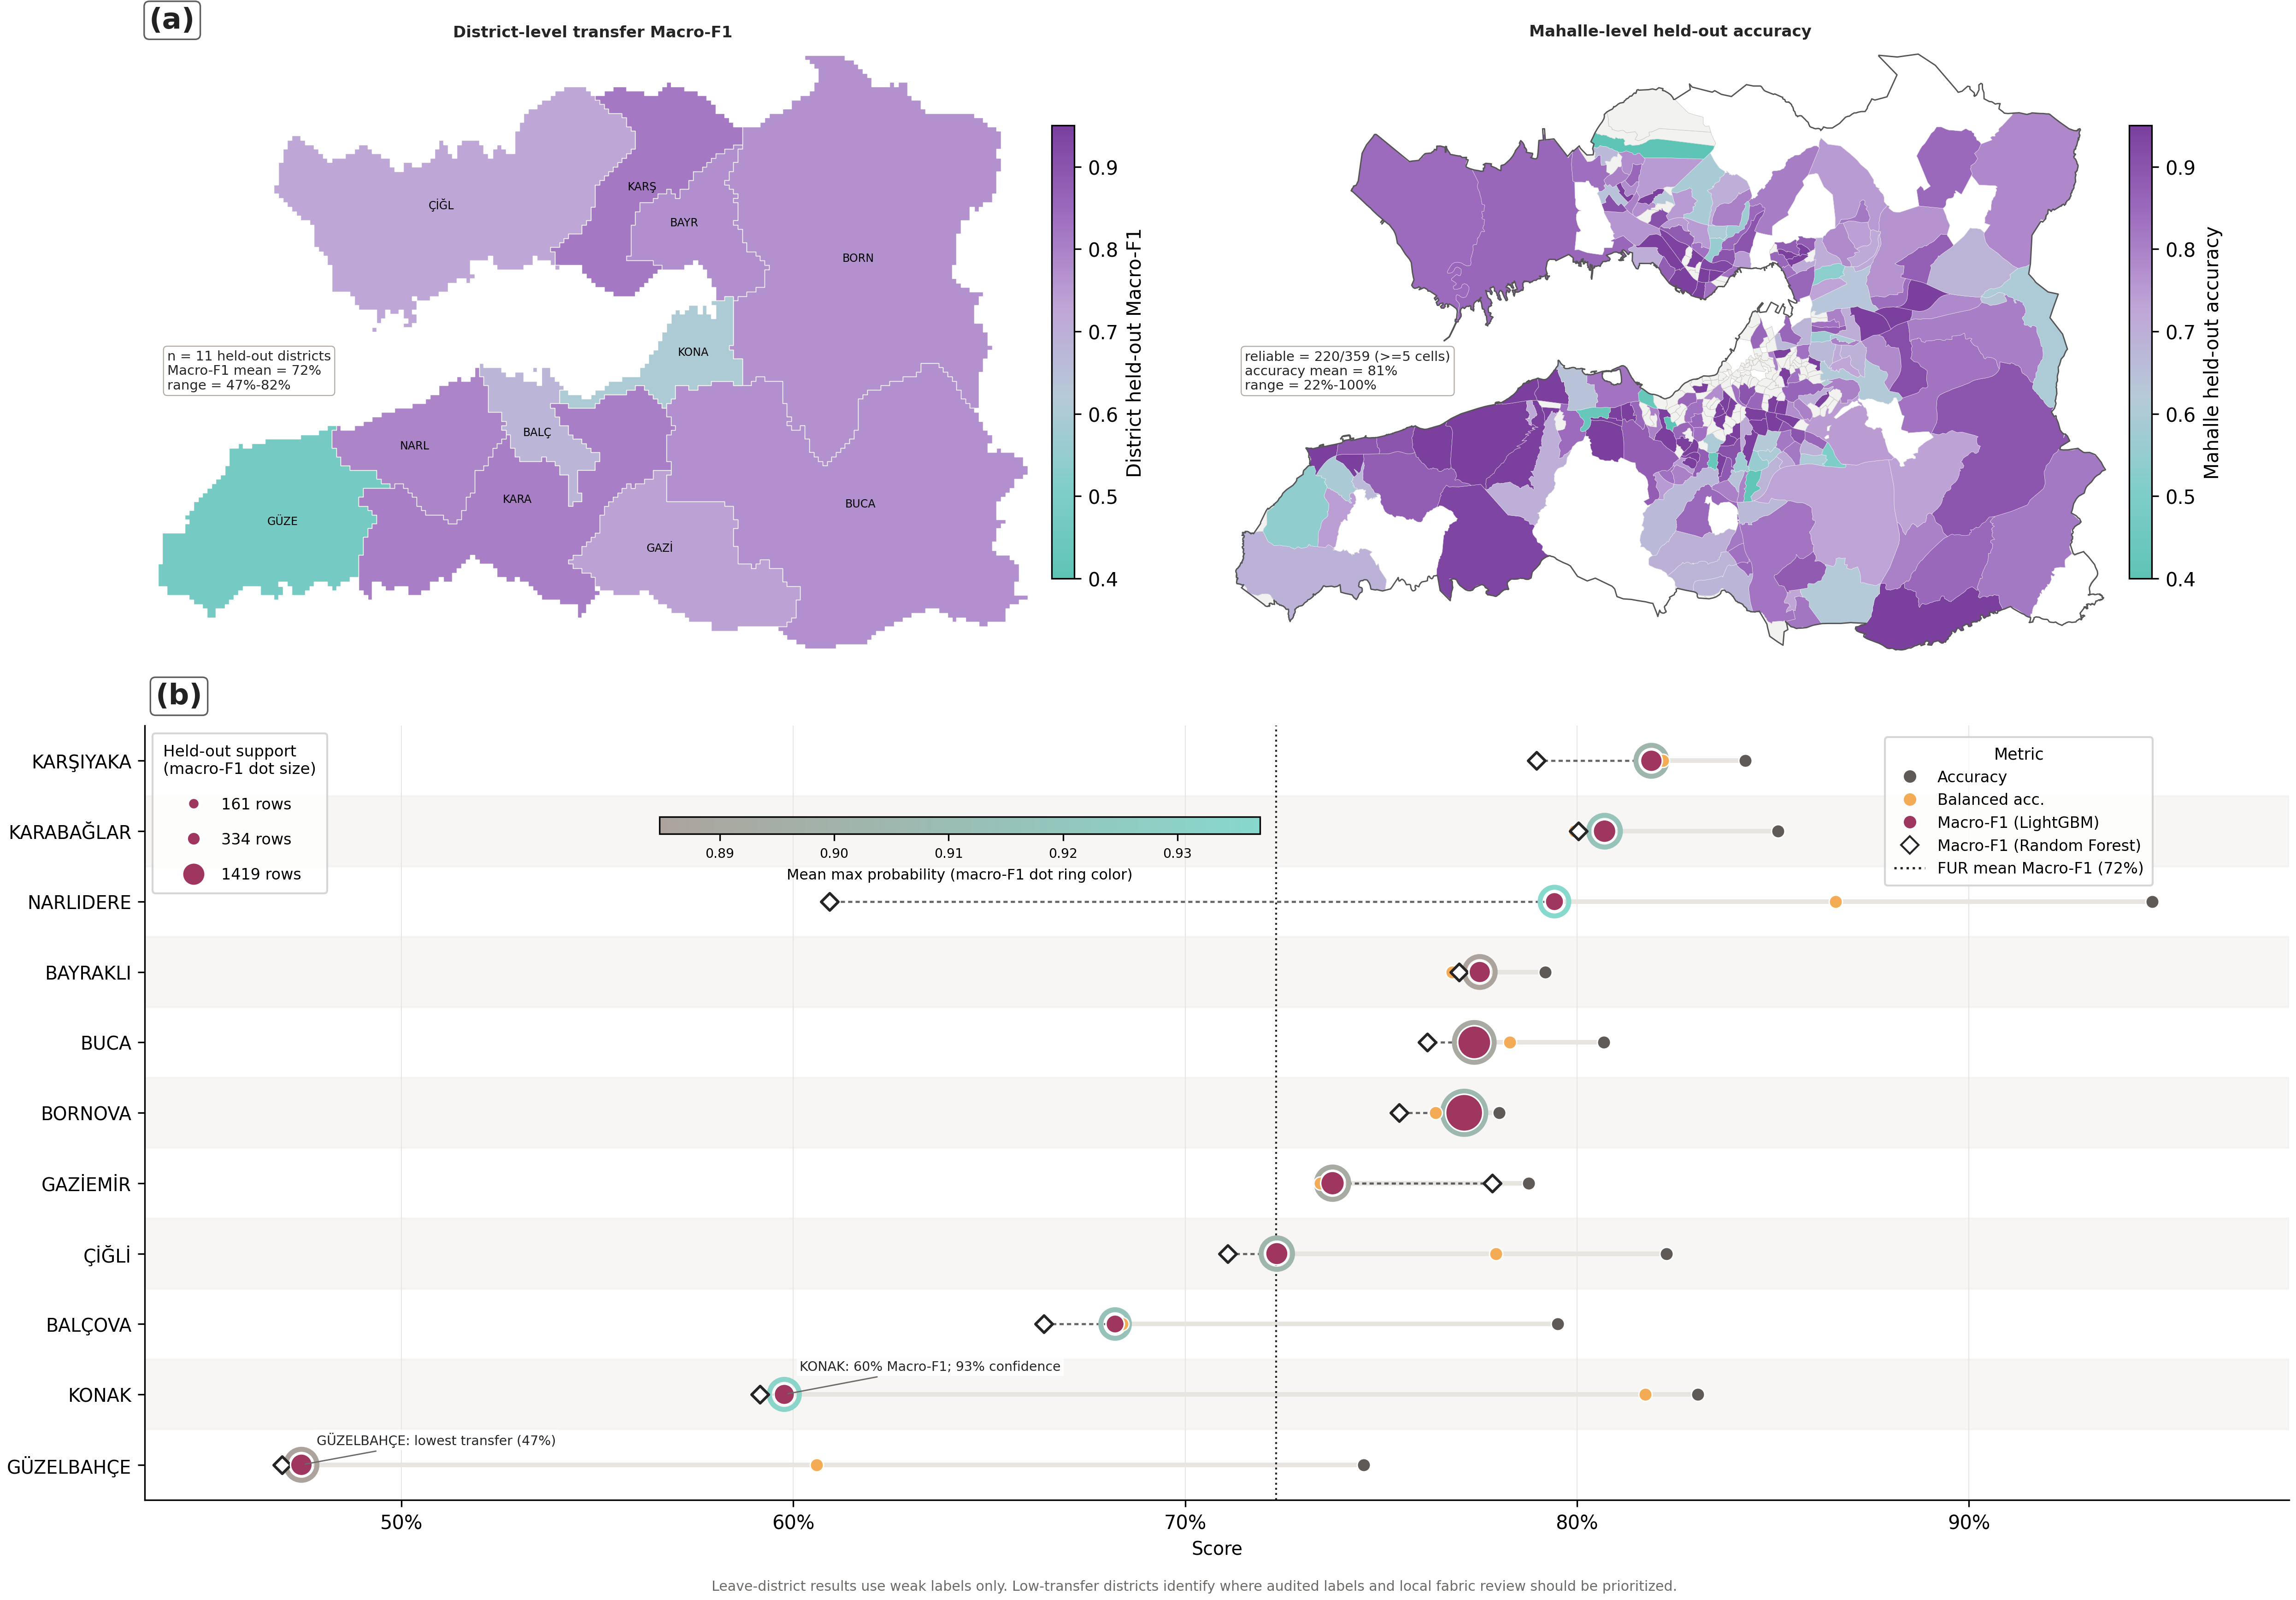
\includegraphics[width=0.9\textwidth]{fig_10_leave_district_out.png}
    \caption{LightGBM leave-one-district-out transfer. Only districts with at
    least 100 eligible observations are included; scores use classes present in each
    held-out district, with Random Forest shown as a comparison in panel (b).}
    \label{fig:lodo}
\end{figure}

\begin{table*}[htbp]
\centering
\footnotesize
\caption{Leave-one-district-out LightGBM weak-label robustness.}
\label{tab:leave_district}
\resizebox{\textwidth}{!}{%
\begin{tabular}{lrrrrr}
\toprule
Held-out district & $n$ & Classes & Accuracy & Balanced accuracy & Macro-F1 \\
\midrule
G\"uzelbah\c{c}e & 334 & 3 & 0.746 & 0.606 & 0.475 \\
Konak & 266 & 3 & 0.831 & 0.817 & 0.598 \\
Bal\c{c}ova & 161 & 4 & 0.795 & 0.684 & 0.682 \\
Cig\u{g}li & 367 & 4 & 0.823 & 0.779 & 0.723 \\
Gaziemir & 438 & 4 & 0.788 & 0.735 & 0.738 \\
Bornova & 1419 & 4 & 0.780 & 0.764 & 0.771 \\
Buca & 1082 & 4 & 0.807 & 0.783 & 0.774 \\
Bayrakli & 322 & 4 & 0.792 & 0.768 & 0.775 \\
Narl\i dere & 169 & 3 & 0.947 & 0.866 & 0.794 \\
Karaba\u{g}lar & 390 & 4 & 0.851 & 0.799 & 0.807 \\
Kar\c{s}\i yaka & 331 & 4 & 0.843 & 0.822 & 0.819 \\
\bottomrule
\end{tabular}%
}
\begin{minipage}{0.96\textwidth}\vspace{2pt}\scriptsize Note: Only districts with at least 100 eligible observations were evaluated. Macro-F1 uses classes present in the held-out district; LightGBM mean 0.723 and range 0.475--0.819. Random Forest, evaluated identically as a comparison baseline, reached mean macro-F1 0.700.\end{minipage}
\end{table*}


\subsection{Climate-response validation}

Summer LST differed across the four weak classes ($H=1592.0$, $p<0.001$,
$\epsilon^2=0.298$, $n=5,337$). LCZ 8 was warmest by median, followed by LCZ 3,
LCZ 9, and LCZ 6. Across grid units, NDBI had the strongest positive bivariate
association with LST ($\rho=0.684$), followed by building coverage
($\rho=0.442$), road density ($\rho=0.374$), and endpoint-derived intersection
density ($\rho=0.342$). NDVI ($\rho=-0.678$) and canopy-volume proxy
($\rho=-0.670$) had the strongest negative associations. Figure~\ref{fig:climate}
and Table~\ref{tab:climate_validation} report the complete selected set.

\begin{figure}[!htbp]
    \centering
    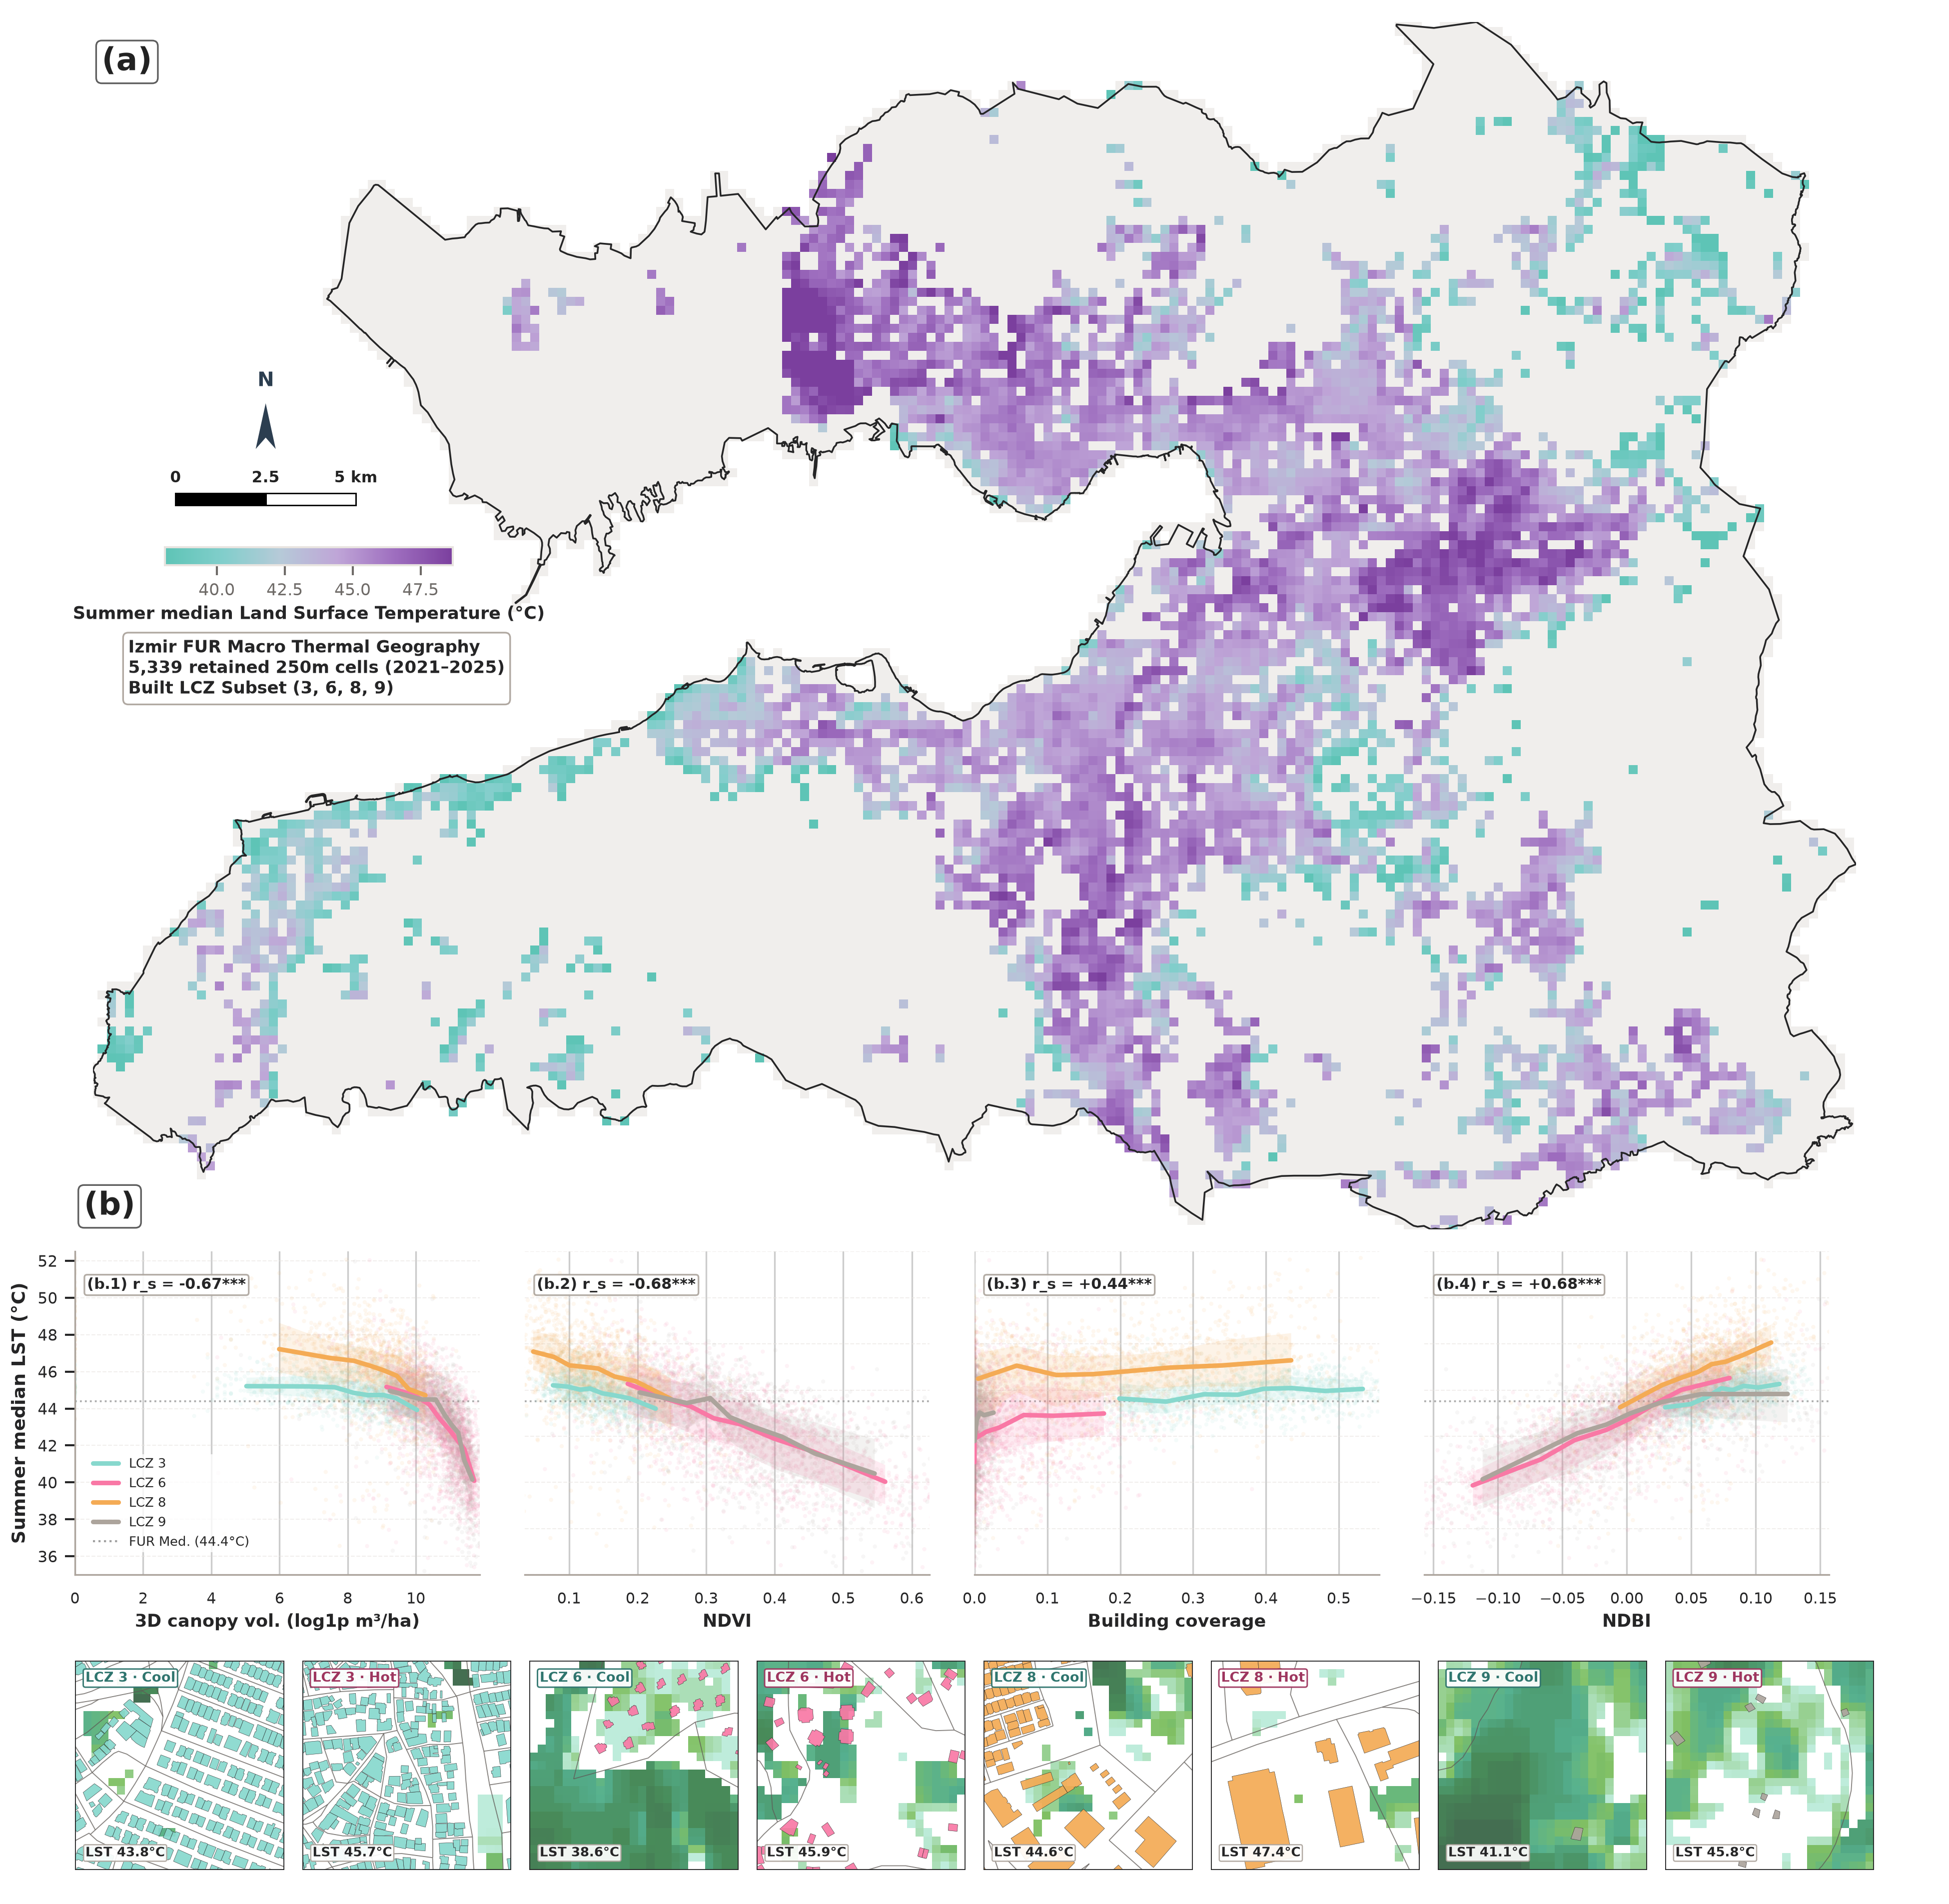
\includegraphics[width=\textwidth]{fig_9_climate_validation.png}
    \caption{Descriptive climate-response validation. (a) Summer median LST by
    weak LCZ class. (b) Spearman correlations between selected features and LST;
    the lower tiles show audited cool/hot contrasts. The statistics are
    cross-sectional and do not estimate causal cooling.}
    \label{fig:climate}
\end{figure}

\begin{table*}[htbp]
\centering
\footnotesize
\caption{Descriptive climate-response associations within the four-class weak-label subset.}
\label{tab:climate_validation}
\resizebox{\textwidth}{!}{%
\begin{tabular}{lrrr}
\toprule
Feature & n & Spearman rho with LST & p \\
\midrule
s2 ndbi mean & 5336 & +0.684 & <0.001 \\
s2 ndvi mean & 5336 & -0.678 & <0.001 \\
canopy volume gt2m proxy m3 per ha & 5337 & -0.670 & <0.001 \\
building coverage exact & 5337 & +0.442 & <0.001 \\
road density exact m per km2 & 5337 & +0.374 & <0.001 \\
network intersection density per km2 & 5337 & +0.342 & <0.001 \\
surface-model elevation m std & 5337 & -0.314 & <0.001 \\
canopy cover gt2m share & 5273 & -0.251 & <0.001 \\
morph open space fragmentation index & 5337 & +0.192 & <0.001 \\
green 2sfca 800m access log1p & 5056 & +0.178 & <0.001 \\
\bottomrule
\end{tabular}%
}
\begin{minipage}{0.96\textwidth}\vspace{2pt}\scriptsize Note: Kruskal-Wallis across LCZ 3/6/8/9: H=1592.0, p<0.001, epsilon-squared=0.298. Associations are bivariate and non-causal.\end{minipage}
\end{table*}



\subsection{Audited-label comparison}

The completed audit exposes a substantial mismatch between the four-class weak
label space and the audited local fabric codebook. In the prespecified
high-quality tier, 96 audited units were available: exact agreement was 8.3\% for the
weak label, 8.3\% for LightGBM, and 9.4\% for Random Forest. The high-plus-medium
sensitivity tier contained 148 audited units, with corresponding agreement of
10.1\%, 12.2\%, and 12.2\%; the all-quality four-class reference contained 165
units, with 10.3\%, 13.3\%, and 13.3\%. Figure~\ref{fig:audited-validation} shows
that many audited natural/open classes are not representable by the four-class
target. These values are therefore evidence of class-space compression and
model transfer limits, not a calibrated estimate of local subtype prevalence.

\begin{figure}[!htbp]
    \centering
    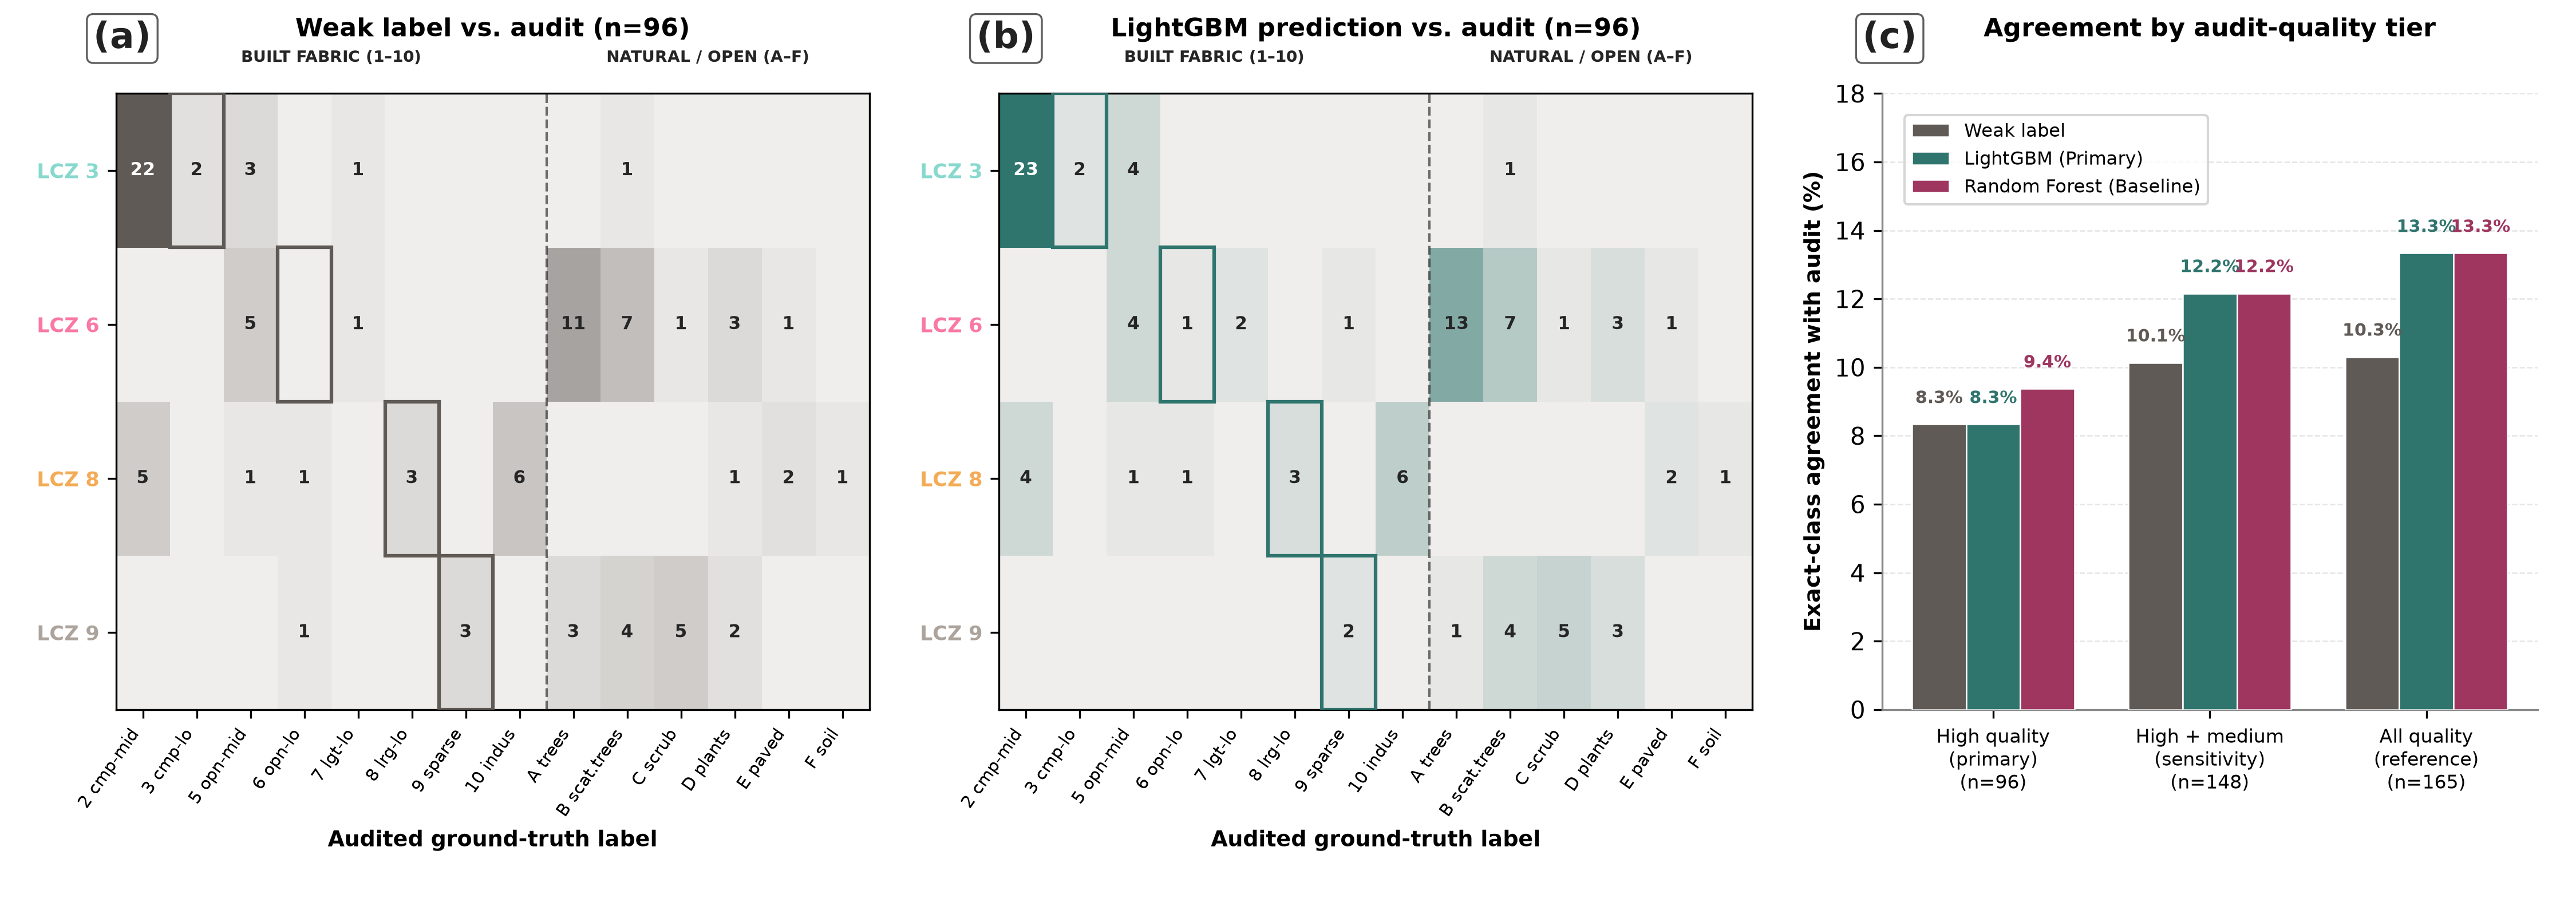
\includegraphics[width=\textwidth]{fig_11_audited_validation.png}
    \caption{Audited-label comparison. (a) Weak label versus audited local
    fabric, (b) LightGBM prediction versus audit, and (c) exact agreement by
    audit-quality tier. The primary tier is the 96-unit high-quality subset;
    agreement is descriptive and natural/open audited classes are retained to
    reveal class-space compression.}
    \label{fig:audited-validation}
\end{figure}

\begin{table*}[htbp]
\centering
\footnotesize
\caption{Manual-audit exact-class agreement for the four-class modeling population.}
\label{tab:audited_validation}
\resizebox{\textwidth}{!}{%
\begin{tabular}{lrrrr}
\toprule
Audit-quality tier & $n$ & Weak label (\%) & LightGBM (\%) & Random Forest (\%) \\
\midrule
High quality (primary) & 96 & 8.3 & 8.3 & 9.4 \\
High + medium (sensitivity) & 148 & 10.1 & 12.2 & 12.2 \\
All quality (reference) & 165 & 10.3 & 13.3 & 13.3 \\
\bottomrule
\end{tabular}%
}
\begin{minipage}{0.96\textwidth}\vspace{2pt}\scriptsize Note: The four-class modeling population is restricted to weak LCZ 3/6/8/9 with confidence $\geq 0.60$. Tiers were prespecified before agreement was computed. The broader unrestricted 569-unit audit had 36.9\% exact weak-label agreement and is not directly comparable to the built-subtype task.\end{minipage}
\end{table*}


\subsection{Claim-status synthesis}

Table~\ref{tab:evidence_status} separates supported, exploratory, and untestable
claims. The study currently supports reproducible data integration,
weak-label discrimination, network-access sensitivity, transfer heterogeneity,
descriptive climate relevance, and bounded audited comparison. It does not
support accurate audited local subtype mapping, deep multimodal superiority, or
planning-ready subtype prescriptions. The low audit agreement is itself a
result, not a basis for filling the remaining claims with extrapolation.

\begin{table}[!htbp]
\centering
\footnotesize
\caption{Analytical evidence summary.}
\label{tab:evidence_status}
\resizebox{\textwidth}{!}{%
\begin{tabular}{lll}
\toprule
Analytical component & Available evidence & Interpretation \\
\midrule
250 m data integration & 16,506 rows, 374 fields, no join loss & supported \\
Surface and context contribution & Surface summaries, ablations, and importance & interpretable contribution \\
Green-space accessibility & network-cost 2SFCA + reference macro audit & proxy supported \\
Spatial robustness & 5 folds + 11 held-out districts & weak-label supported \\
Climate relevance & LST class contrast and correlations & descriptive supported \\
Audited LCZ refinement & 569/569 complete; primary agreement 8.3\% (weak) and 8.3\% (LightGBM) & direct audit comparison \\
CLIMORFA multimodal design & raster, figure-ground, and tabular branches with branch-wise attribution & extensible architecture \\
\bottomrule
\end{tabular}%
}
\begin{minipage}{0.96\textwidth}\vspace{2pt}\scriptsize Note: The summary distinguishes the empirical components of the present analysis from the architecture designed for multimodal extension.\end{minipage}
\end{table}


    \section{Discussion}\label{sec:discussion}

\subsection{What the evidence-grounded baseline establishes}

The principal result is not a new local LCZ map. It is the demonstration that a
locally assembled, interpretable evidence stack materially improves
spatially independent discrimination of global weak labels while the completed
audit exposes where those labels fail to represent local fabric. Morphology
alone carries substantial signal, but vegetation adds the largest early gain,
followed by green-blue and broader proxy context. This supports the literature's
move from class labels toward multidimensional urban form and vegetation structure
\citep{zhou2022UnderstaEffects,wang2023EffectivFactors,
bai2025ImpactBuilding,yu2026UrbanMorpholo}. At the same time, the importance of
WorldCover and Dynamic World variables warns that global land-cover semantics
may partly reproduce the target's own remote-sensing logic. The full-model
score cannot therefore be interpreted as purely independent local morphology.

The local 5 m surface model contributes surface roughness and relief at a much finer
resolution than the LCZ weak-label raster. Its scientific value lies in the
combination with exact footprints, floor-count proxies, and vegetation, not in
a claim that surface-model values are direct building heights. This distinction is
important because SVF and 3D urban-form studies demonstrate both the value and
the scale dependence of surrounding surface geometry
\citep{chen2010ViewFactor,middel2018ViewFactor,
wu2025ContrastUrban,yu2026UrbanMorpholo}. In Izmir, LCZ 3 combines high coverage
and vertical intensity, whereas LCZ 8 combines large-footprint form with the
highest median LST. These patterns are physically plausible, but only a manual
label audit can determine whether they represent locally coherent fabrics or
weak-label mixtures.

\subsection{Why 2SFCA is preferable to a green-space buffer}

The 2SFCA experiment changes the meaning of context. A Euclidean buffer answers
how much mapped green area lies within a circle. Network 2SFCA instead asks how
much supply is reachable through a road-cost graph after accounting for demand
competition. This is closer to an accessibility construct and avoids implying
that distance alone equals service. The positive primary-recipe increment for
LightGBM is modest and model-dependent, showing that the resulting field adds
some signal beyond local morphology and green-blue cover without becoming a
standalone accessibility measure.

Threshold results reinforce the need for sensitivity rather than a single
``correct'' catchment. LightGBM was marginally strongest at 1,200 m, whereas
the preregistered 800 m threshold remained positive across the primary model
comparison. Such
model dependence is expected when urban-form and temperature relationships
change with spatial support \citep{wu2022ScaleEffect,jeon2023ImpactsUrban,
li2026InvestigEffect}. We retain 800 m as the primary planning-scale proxy and
report the other thresholds rather than choosing the best after observing the
outcome. This avoids turning sensitivity analysis into hidden hyperparameter
optimization.

The municipal park comparison provides a useful but bounded validation. Strong
log-count and log-area correlations indicate that OSM supply follows the broad
district geography of the official maintenance inventory. Lower rank
correlations, sparse OSM names, and only 10.6\% exact-or-strong name candidates
show why this cannot validate individual polygons, public access, quality, or
completeness. The 2SFCA should therefore be interpreted as mapped green-supply
access, not a service-equity score.

\subsection{Spatial transfer is the central reviewer test}

Five spatial block folds produce stable average performance, but the LightGBM
LODO test reveals a 0.344 range in macro-F1. The hard transfers are not random noise; they
are evidence that district-specific combinations of coast, slope, building
stock, function, and label composition matter. The 0.115 difference between
mean spatial-fold and mean district-held-out macro-F1 is therefore more
informative than another decimal place in the headline score. It shows how a
model can interpolate local structure while struggling when an administrative
and morphological context is entirely absent from training.

This finding agrees with work showing that LCZ thermal meaning and urban-form
relationships vary across city, season, class, and analytical unit
\citep{kwok2019WellDoes,deng2024SensitivLocal,
wang2025SeasonalEffects,wu2025ContrastUrban}. A future external-city test would
be even harder. Before that step, the Izmir audit should oversample or at least
carefully inspect the districts with low LODO scores, while preserving the
original probability sample for unbiased reporting.

\subsection{Climate relevance and planning interpretation}

The LST contrast provides climate relevance without making LST a predictor.
The large Kruskal effect size and the warm LCZ 8 profile indicate that broad
weak-label fabric categories organize surface temperature. The correlation pattern is also
internally coherent: NDBI, building coverage, and road density are positive,
whereas NDVI and canopy volume are negative. Similar studies show that
morphology and vegetation effects can vary by LCZ, season, and scale
\citep{zhou2023IdentifyEffects,liu2025UnveilinDifferen,
wang2025SeasonalEffects}. Our bivariate results should not be converted into
causal prescriptions such as a fixed percentage of canopy producing a fixed
cooling benefit.

Planning translation should therefore be conditional. In large low-rise,
high-LST fabrics, priorities may include roof and yard heat mitigation,
continuous tree shade, and reducing exposed impervious service areas. In
compact low-rise fabrics, street-canyon shade, ventilation-sensitive planting,
and small-networked green spaces may be more relevant than large isolated
parks. In open low-rise and sparsely built areas, retaining vegetation and
preventing fragmentation may be more important than blanket densification.
These are mechanism-informed hypotheses for audited subtype panels, not current
policy prescriptions.

Nor does morphology equal vulnerability. LCZ and LST organize exposure, but
heat risk also depends on social sensitivity, mobility, occupation, housing,
and adaptive capacity \citep{ma2023InvestigUrban,mashhoodi2024UrbanForm,
iqbal2025DoesPerceive,turner2025DevelopmValidati}. The present model contains no
individual vulnerability data and should not be used to rank populations.
Future planning synthesis can join audited climate-morphology types to
area-level vulnerability only with separate governance, denominator, and
privacy checks.

\subsection{What a deep model must add}

A deep model is justified only if it extracts spatial configuration not already
captured by 68 tabular predictors. Figure-ground texture, street-building
interface, vegetation placement, and localized surface-model patterns are plausible
sources of additional information. Prior LCZ and urban-fabric work demonstrates
that CNN and multi-view representations can learn such structure
\citep{qiu2020MultilevFeature,yoo2020ImprovinLocal,
fang2024UrbanclaDeep}. But superiority must be established through identical
spatial folds, audited labels, branch ablations, probability calibration, and
attribution. A higher weak-label score without these checks would merely learn
the global label product more efficiently.

The current stopping rule is therefore a strength. It prevents a planned
architecture from being described as an implemented contribution. The completed
audit already shows that weak-label agreement is only 8.3\% in the primary
high-quality tier, so the key next test is not whether CLIMORFA beats Random
Forest by any weak-label margin, but whether raster and figure-ground branches
improve audited transfer, reduce systematic uncertainty, and reveal
interpretable subtype structure. SHAP and neural attributions must agree at the level of mechanism
families rather than being selected as decorative examples
\citep{xu2025CharacteThermal,han2025PerspectUndersta,
liu2026UnderstaNonlinea}.

\subsection{Limitations}

First, all classification results use global weak labels and four represented
built classes. The confidence threshold removes some uncertainty but can also
select easier, more homogeneous examples. Second, the manual audit is complete,
but the primary high-quality comparison contains only 96 four-class modeling
units and shows low agreement; it should not be generalized to a complete local
subtype census.
Third, the 5 m surface model is a surface model with uncertain vertical datum and no
terrain normalization, while floor-count height is a proxy. Fourth, Landsat LST
is a summer surface-temperature composite, not air temperature, thermal comfort,
or personal exposure. Fifth, missingness is partly structural, and median
imputation may blur the distinction between absence and unknown data.

Sixth, OSM functional context is not official zoning, and OSM park/garden supply
is neither a complete green inventory nor proof of access. The 2SFCA graph is
based on municipal road centrelines, not a fully audited pedestrian network;
explicit motorways were removed, but ramps or grade-separated segments may
remain under other codes. Seventh, endpoint-derived network measures are not a
fully planar topological graph, and street-frontage fields are road-buffer
proxies. Eighth, 500 m data are prepared but the complete 500 m model comparison
and optimized 125 m pipeline have not run. Finally, feature importance is
model-specific, correlations are bivariate, and no causal effect is estimated.

These limitations define a finite completion path: train raster and
figure-ground branches on identical audited spatial folds; run 125/250/500 m
analyses; calibrate uncertainty; perform branch-level XAI; and repeat the
climate and planning synthesis only for audited subtypes. The completed audit
is now an input to that next stage rather than an outstanding data gate.


    \section{Conclusions}\label{sec:conclusions}

This study assembled a reproducible climate-morphology evidence frame for the
Izmir functional urban region and tested what can be learned from global weak
labels plus a completed local audit. A 250 m matrix covering 16,506 grid units
integrates a
local 5 m surface model, exact building and street geometry, vegetation
structure, remote sensing, coast, OSM context, population demand, and
network-cost green-space accessibility. Under five spatial block folds, the
primary 800 m LightGBM reached weak-label macro-F1 0.838, compared with 0.663
for morphology alone. Vegetation produced the largest additive gain, 2SFCA
contributed a modest model-dependent increment, and leave-district-out
performance exposed substantial geographic transfer loss. Weak classes also
showed a large LST contrast and coherent vegetation/built-form associations.

The methodological conclusion is stronger than any single score. LCZ labels are
most useful here as a common vocabulary and sampling scaffold, not as local
ground truth. Fine surface-model information, 3D vegetation, network
accessibility, spatial validation, audit comparison, and explicit proxy language
make that scaffold more planning-relevant and more falsifiable. Euclidean buffers would not represent
the same accessibility construct as 2SFCA, and random splits would not reveal
the district transfer problem.

CLIMORFA therefore provides a reproducible multimodal evidence framework whose
tabular branch is evaluated against spatial folds and a completed manual audit.
The 8.3\% agreement in the primary high-quality four-class population is an
important finding: it identifies class-space compression that should inform
future local subtype work. The architecture, branch comparisons, attribution
tools, calibrated uncertainty, and multi-scale analysis provide a coherent path
for extending the evidence base while retaining the same audit and spatial-
validation principles.

    \section*{CRediT authorship contribution statement}

The final CRediT statement will be confirmed by Yusuf Emino\u{g}lu, Mert
Yava\c{s}, Hilmi Evren Erdin, and \c{S}\i rk\i before journal submission.
Conceptualization, methodology, software, validation, formal analysis,
investigation, resources, data curation, writing, visualization, supervision,
project administration, and funding acquisition will be assigned only to
contributors who meet the journal's authorship criteria.

\section*{Declaration of competing interest}

The authors declare that they have no known competing financial interests or
personal relationships that could have appeared to influence the work reported
in this paper. This statement must be reconfirmed by every named author at
submission.

\section*{Funding}

Funding information, including grant numbers and funder roles if applicable,
will be confirmed by the authors before journal submission.

\section*{Data and code availability}

Processing scripts, parameter manifests, derived tables, figures, and audit
protocols are organized in the public project repository at
\url{https://github.com/YusufEminoglu/climorfa}. The repository includes a
versioned code archive, environment information, derived non-restricted metrics
where licensing permits, and provenance for external inputs. The local surface
model, Akilli Sehir data, and any other restricted inputs are not redistributed
without explicit permission; instead, provenance, schema, processing code, and
reproduction instructions are supplied. Public Earth-observation and OSM
sources are referenced with access date and source URL. A permanent DOI will be
added if the repository is archived.

\section*{Ethics and privacy}

The analysis uses gridded environmental, building, road, land-cover,
and aggregate neighbourhood population data. It contains no individual-level
records. Any later linkage to vulnerability or mobility data requires a separate
privacy, denominator, and ethics review.

\section*{Declaration of generative AI and AI-assisted technologies}

AI-assisted tools were used during code and manuscript development under human
supervision. They were not treated as authors, data sources, or validators.
All numerical claims are linked to executable scripts and
machine-readable outputs. The wording of this declaration must be aligned with
the target journal's policy at submission.


    \clearpage
    \section*{List of Abbreviations}
    \begin{description}
        \item[2SFCA] Two-step floating catchment area
        \item[CLIMORFA] Climate-Morphology Fusion Architecture
        \item[FUR] Functional urban region
        \item[LCZ] Local Climate Zone
        \item[LODO] Leave-one-district-out
        \item[LST] Land-surface temperature
        \item[NDVI] Normalized Difference Vegetation Index
        \item[NDBI] Normalized Difference Built-up Index
        \item[NDWI] Normalized Difference Water Index
        \item[OOF] Out-of-fold
        \item[OSM] OpenStreetMap
        \item[RF] Random Forest
        \item[SVF] Sky-view factor
        \item[WUDAPT] Worldwide Urban Database and Access Portal Tools
        \item[XAI] Explainable artificial intelligence
    \end{description}

    \clearpage
    \bibliography{refs}

    \clearpage
    \appendix

\section{Supplementary diagnostics and reproducibility evidence}\label{sec:appendix}

This appendix contains the current evidence-bearing diagnostics used to
interpret the weak-label baseline. It is limited to reproducible feature,
surface-model, canopy, and spatial-fold evidence. Retired
external-triangulation diagnostics, duplicate weak-label panels, manual-audit
figures, and untrained deep-model outputs are not part of the supplementary
bundle; the completed audit is reported in the main text.

All panels were generated from the locked feature matrix and model-output
directories identified in the project figure map. Source paths, parameters,
selection rules, and claim boundaries are retained in the accompanying
manifests and build scripts.

\subsection{Matched urban-texture, surface-model, and canopy atlas}

The atlas contains the same 48 deterministic selection cells used for the
within-class climate--morphology comparison. Each cell is shown through
matched figure-ground texture, surface-model elevation/roughness, and cleaned
10 m canopy-height views. The atlas is descriptive and reproducible from the
exported selection manifest; it is not an audited local subtype validation.

\begin{figure*}[htbp]
    \centering
    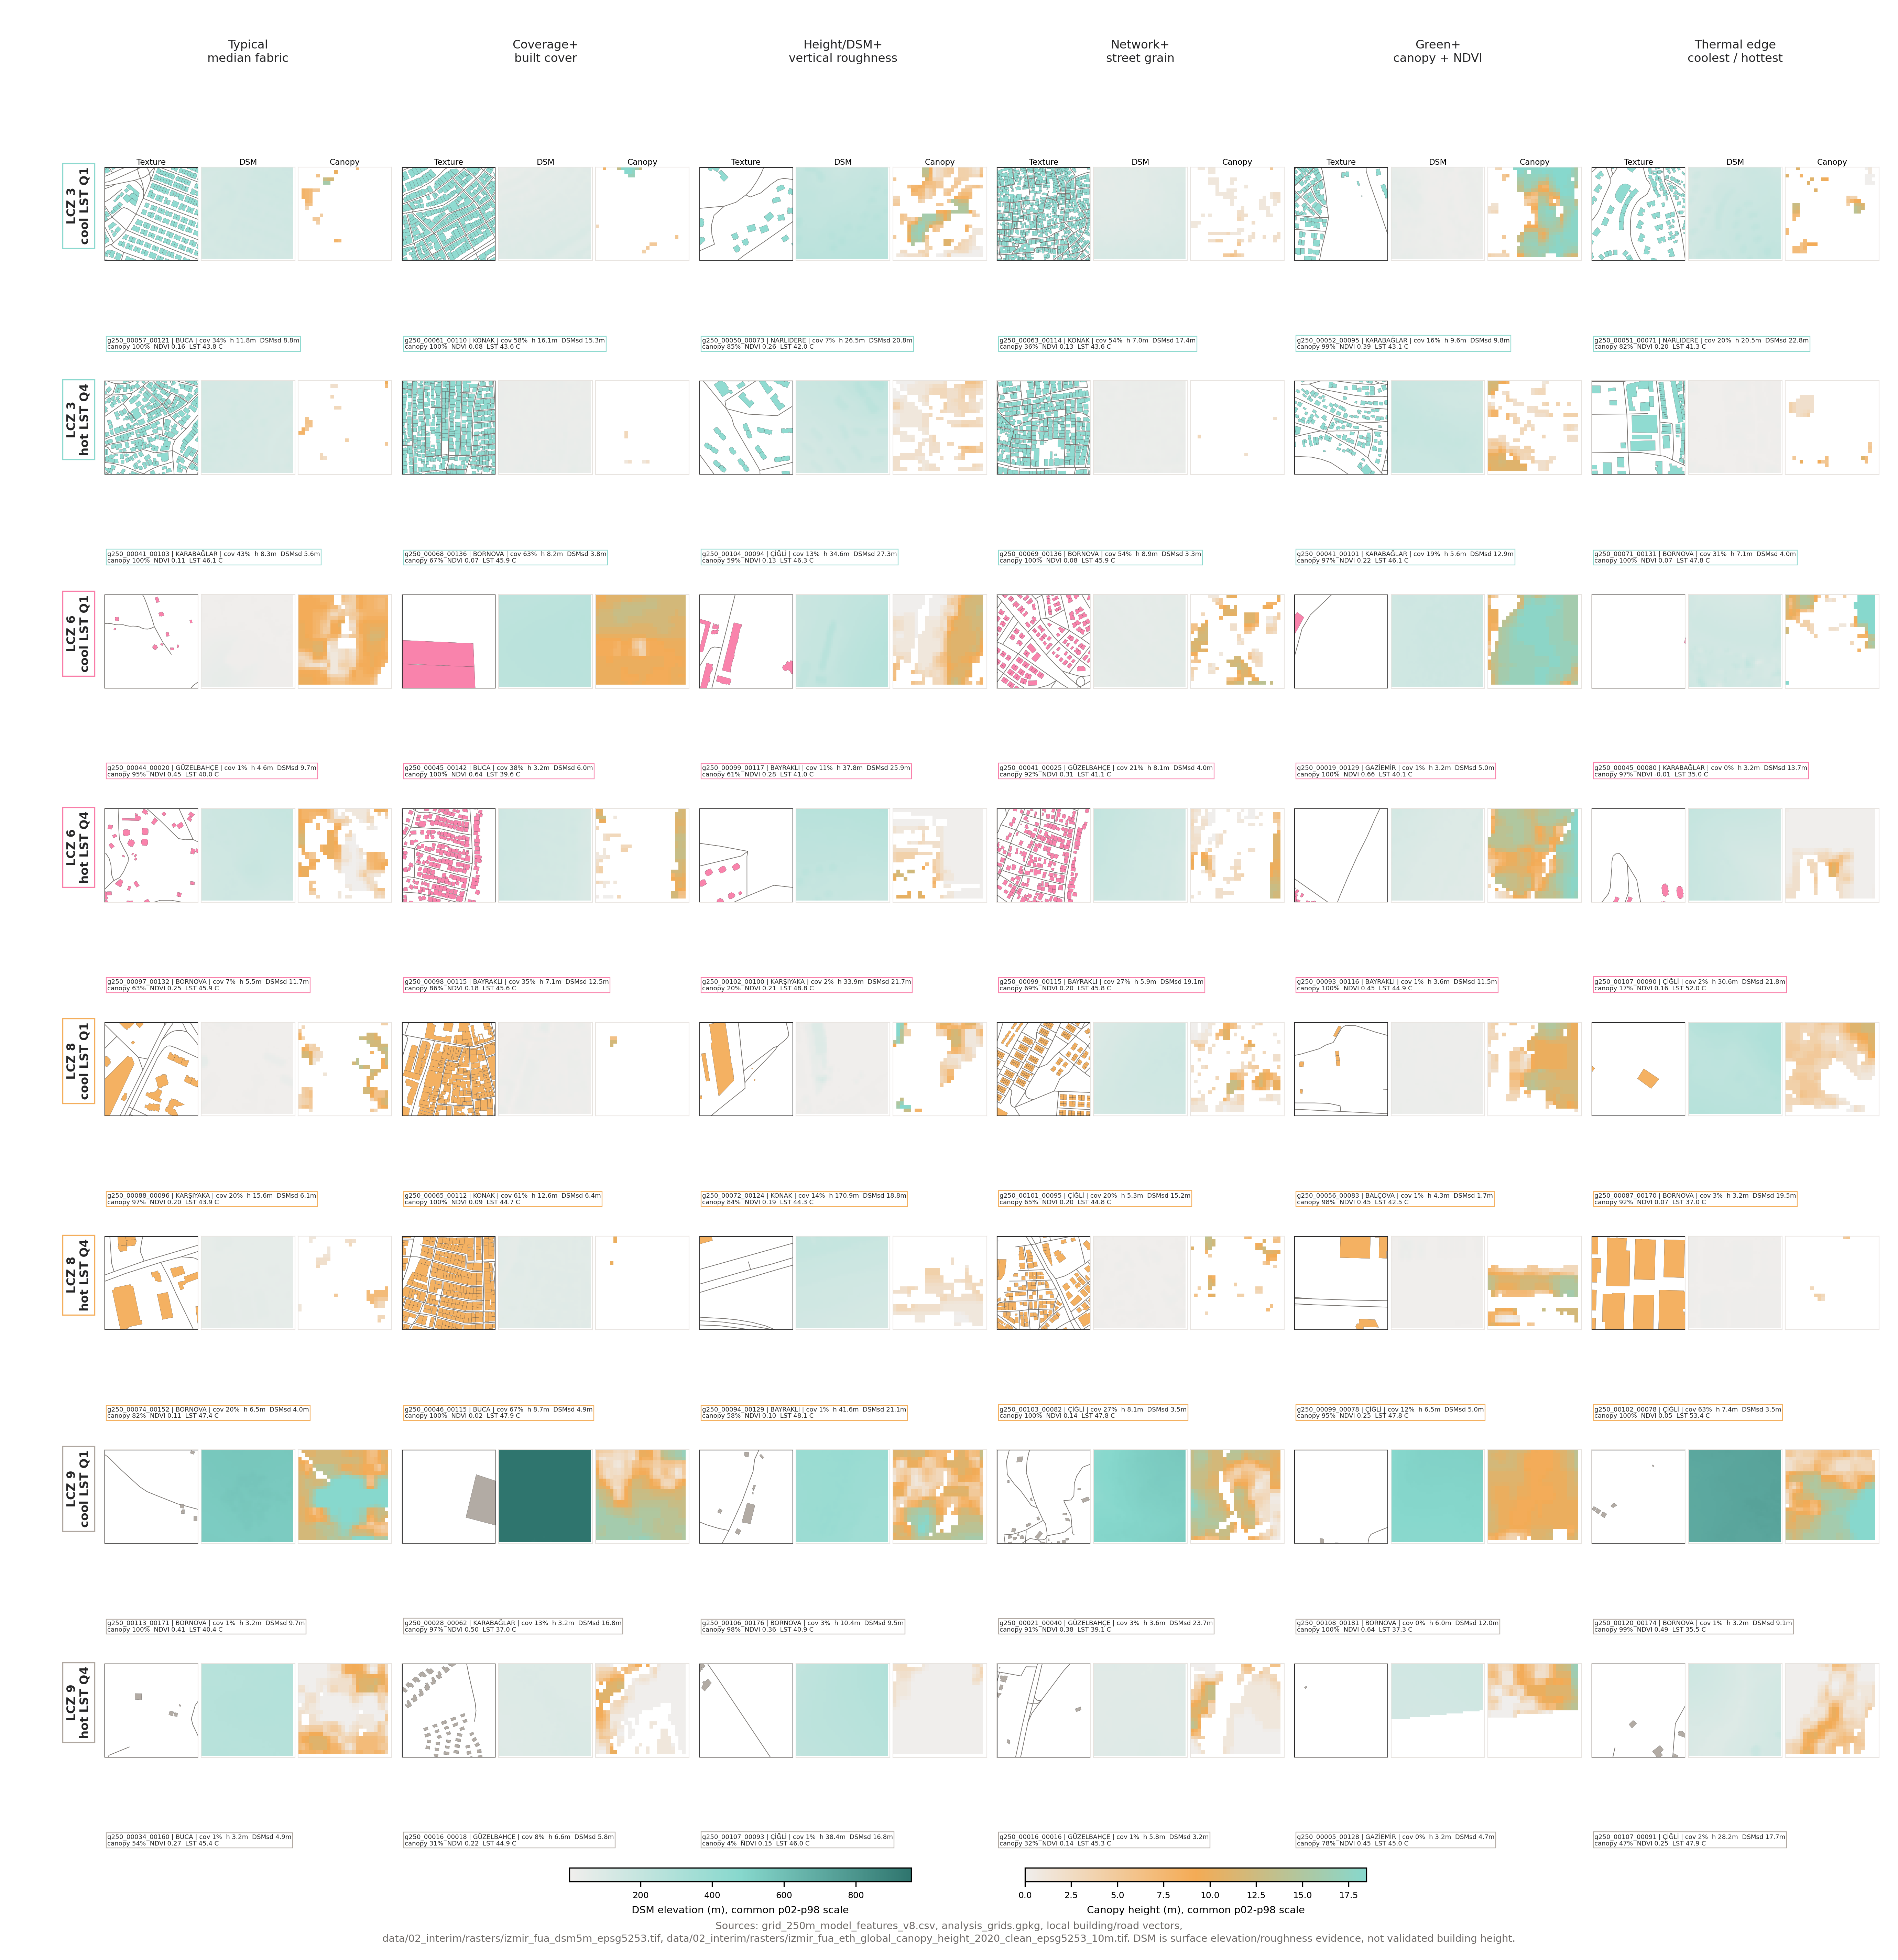
\includegraphics[width=\textwidth]{fig_s1_texture_dsm_canopy_atlas_48_cells.png}
    \caption{Matched 48-cell urban-texture atlas. Each selected cell contains
    figure-ground texture, surface-model elevation/roughness, and canopy-height
    views on shared robust scales. The figure is a visual evidence bridge, not
    a validated building-height or audited local-classification result.}
    \label{fig:s1-texture-surface-canopy}
\end{figure*}
\FloatBarrier

\subsection{Feature quality and collinearity}

Feature missingness is interpreted together with structural-absence flags
before fold-specific imputation. The collinearity panel records the largest
groups at absolute correlation $r\geq0.95$; family-level ablations and
representative variables are used to reduce redundancy in the reported
baselines.

\begin{figure*}[htbp]
    \centering
    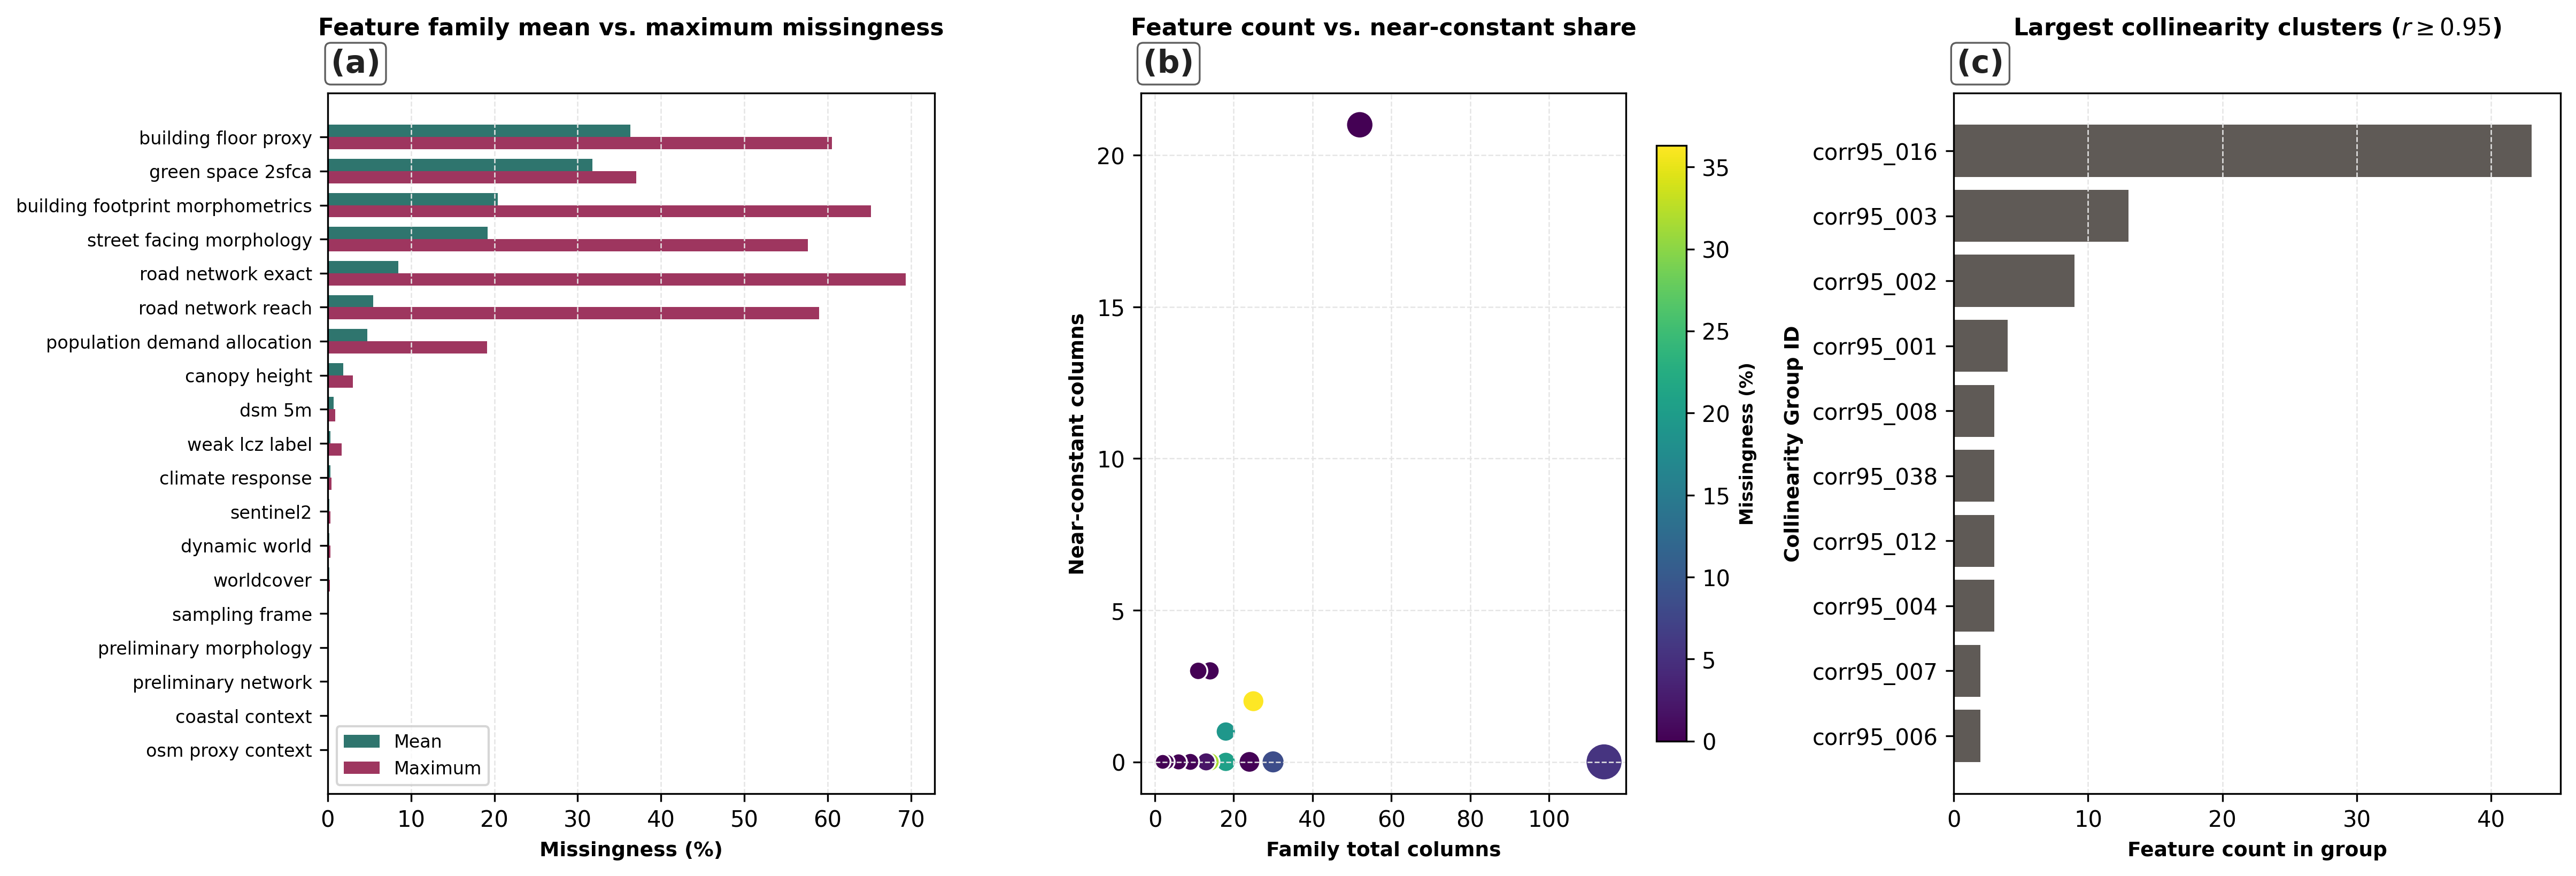
\includegraphics[width=0.96\textwidth]{fig_s2_feature_quality.png}
    \caption{Feature-quality diagnostic. (a) Mean and maximum missingness by
    family, (b) feature count versus near-constant columns, and (c) the largest
    high-correlation feature groups.}
    \label{fig:s2-feature-quality}
\end{figure*}
\FloatBarrier

\subsection{Spatial-fold diagnostics}

The primary spatial folds are fixed before model comparison. This diagnostic
shows class support by fold and the fold-wise distribution of the primary
LightGBM out-of-fold prediction probability. It is a stability diagnostic for
the weak-label baseline and does not constitute audited subtype validation.

\begin{figure*}[htbp]
    \centering
    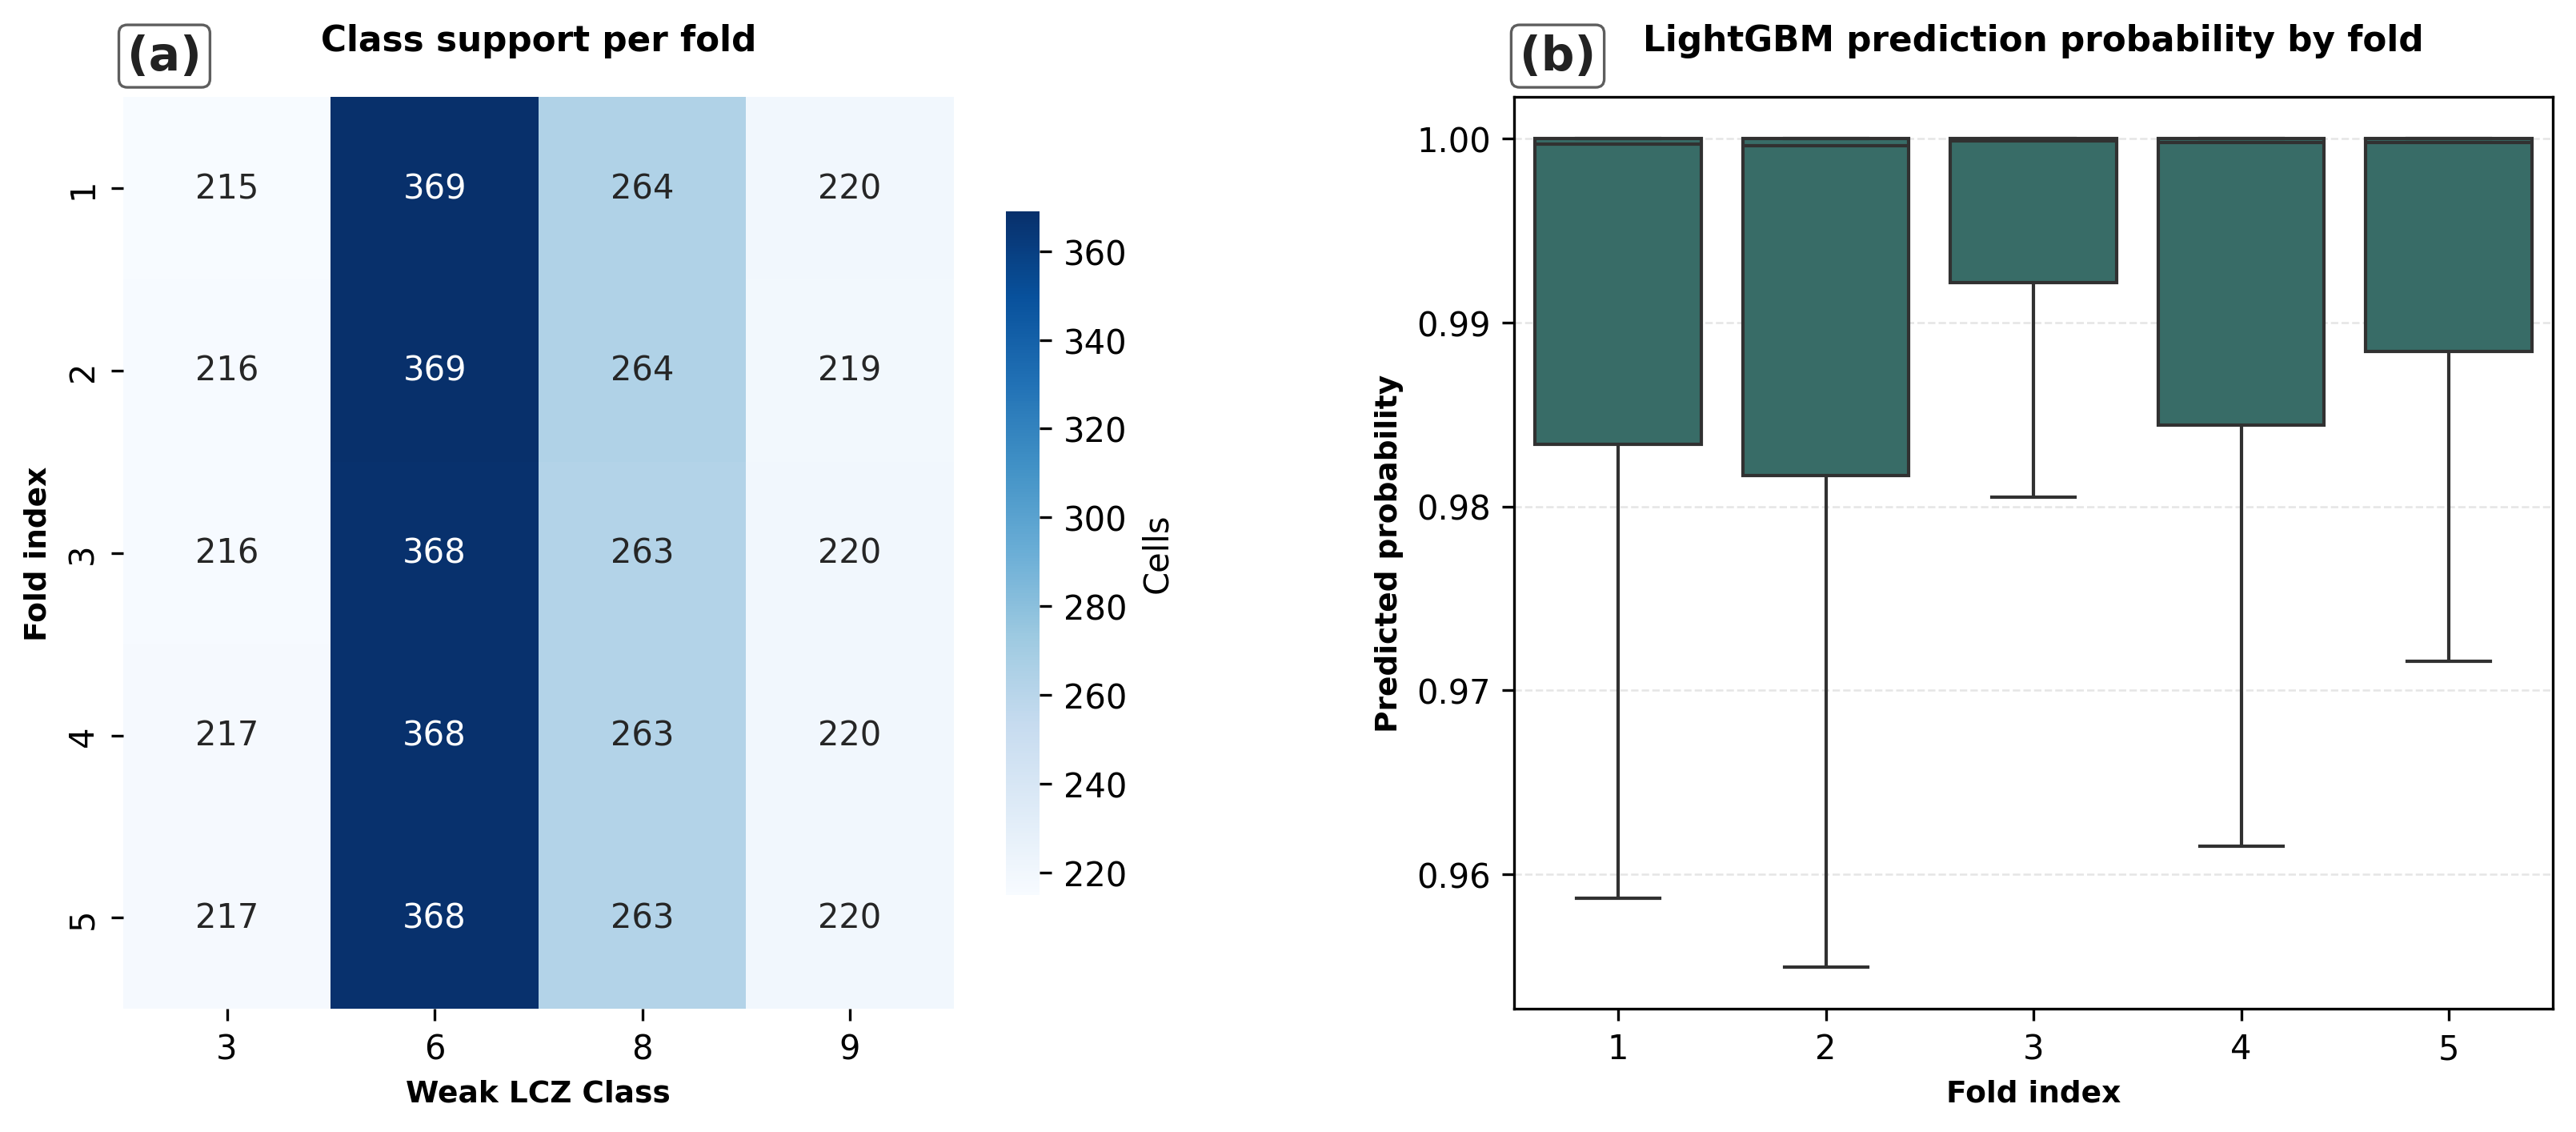
\includegraphics[width=0.92\textwidth]{fig_s3_spatial_fold_diagnostics.png}
    \caption{Spatial-fold diagnostics. (a) Weak-class support across the fixed
    spatial folds and (b) primary LightGBM out-of-fold prediction probability
    by fold.}
    \label{fig:s3-spatial-folds}
\end{figure*}
\FloatBarrier

\subsection{Reproducibility checklist}

The analysis package should be considered internally reproducible when the
following checks pass: (i) the v8 input has 16,506 rows and 374 fields; (ii)
all manifest-referenced fields exist; (iii) the four-class filter returns
5,339 rows; (iv) every eligible row has one spatial fold; (v) preprocessing is
fitted inside training folds; (vi) all reported out-of-fold outputs are
regenerated from the locked scripts and parameters; and (vii) the PDF compiles
without missing figure, table, citation, or reference warnings. The manual
audit is complete, but deep multimodal fusion remains unavailable until its
output manifests exist, so no supplementary panel should be read as evidence
of a trained deep model.


\end{document}




